%%%%%%\documentclass{beamer}
%%%%%%\usepackage{hyperref}
%%%%%%\usepackage{subfig}  %% Para incluir subgraficos
%%%%%%\usepackage{graphicx}
%%%%%%\usepackage{media9} % 
%%%%%%\usepackage{url}
%%%%%%\usepackage{ragged2e}  % Allow justification
%%%%%%\usepackage[margin=20pt,font=small,labelfont=bf,labelsep=period]{caption}
%%%%%%
%%%%%%\usepackage[spanish, activeacute]{babel}
%%%%%%\usepackage[utf8]{inputenc}
%\pdfminorversion=5 % To enforce 1.5 version of PDF
% Tipo de documento
% ***********************************************
% ***********************************************
\documentclass[xcolor=table]{beamer} %[draft]

% No lo he trabajado bien
% ***********************************************
%\usepackage{handoutWithNotes}
%\pgfpagesuselayout{2 on 1 with notes landscape}[a4paper,border shrink=5mm]

% Cargando paquetes
% ***********************************************
\usepackage[english]{babel}
%\usepackage[latin1]{inputenc}
%\usepackage[spanish, activeacute]{babel}
%\usepackage[spanish]{babel}
\usepackage[utf8]{inputenc}

%Juan Carlos Vergara Gallego
%%%%%\documentclass{beamer}
\usepackage{hyperref}
\usepackage{subfig}  %% Para incluir subgraficos
\usepackage{graphicx}
\usepackage{media9} % 
\usepackage{url}
\usepackage{ragged2e}  % Allow justification
\usepackage[margin=20pt,font=small,labelfont=bf,labelsep=period]{caption}


% Templates beamers
% ***********************************************
\usetheme[compress]{Dresden}
%\usecolortheme{dolphin}
\setbeamercovered{transparent}
%\usefonttheme[onlymath]{serif}
\usefonttheme[onlysmall]{structurebold}
%\usefonttheme{serif}
\beamertemplatenavigationsymbolsempty
\useinnertheme[shadow=true]{rounded}


% Más paquetes
% ***********************************************
\usepackage{color}
\usepackage{colortbl}
\usepackage{ziffer}
\usepackage{amsmath, amssymb}
\usepackage{etex}
\usepackage[absolute,overlay]{textpos}
\usepackage{framed}
\usepackage{multimedia}

\usepackage{decimal}
\usefonttheme{serif}  % Make equations to be in serif fonts
%\decimalpoint


\hypersetup{pdfstartview={Fit}, bookmarks=True, pdftitle={SCEC Presentation}, pdfauthor={Juan Carlos Vergara-Gallego}, pdfsubject={Presentation}, pdfkeywords={Waves, Elasticity, Numerical Methods, High Performance Computing, BEM}, pdfpagemode=UseOutlines, bookmarks, bookmarksopen, pdfstartview=FitH, colorlinks,linkcolor=blue, urlcolor=black, citecolor=blue}  % Configure hyperref

%--- New commands ----%
\newcommand{\footref}[1]{\textsuperscript{\ref{#1}}}
\newcommand{\pardiff}[2]{\frac{\partial #1}{\partial #2}}
\newcommand{\pardiffd}[2]{\frac{\partial^2 #1}{\partial #2^2}}




% Definitions
% ***********************************************
\setlength{\TPVertModule}{\paperheight}
\setlength{\TPHorizModule}{\paperwidth} 
\setlength{\TPHorizModule}{\paperwidth}\setlength{\TPVertModule}{\paperheight}

\setbeamercolor{footlinecolor}{bg=grayJuan,fg=blueEAFIT}
%\setbeamercolor{footlinecolor}{bg=yellowEAFIT,fg=blueEAFIT} %Define el color de la banda inferior


% Información que va en la franja inferior
%sep: define el alto de la franja inferior
\setbeamertemplate{footline}{%
  \begin{beamercolorbox}[sep=.15em, wd=\paperwidth,leftskip=0.4cm,rightskip=0.4cm]{footlinecolor}
  \mbox{
	\begin{minipage}{0.2\paperwidth}
		
\includegraphics[width=0.1\paperwidth]{img/logo2.pdf}
	\end{minipage}
	\begin{minipage}{0.7\paperwidth}
		\begin{center}
			Juan Carlos Vergara Gallego. -- Mecánica Aplicada
		\end{center}
	\end{minipage}
	\begin{minipage}{0.1\paperwidth}
		\scriptsize{\insertframenumber}
	\end{minipage}}
  \end{beamercolorbox}%
}


% Definiendo los colores
% ***********************************************
\definecolor{grayJuan}   {HTML}{e6e4e4}
%\definecolor{blueEAFIT}   {HTML}{003560}
\definecolor{grenJuan}  {HTML}{94c11c}
\definecolor{middlegray}{rgb} {0.5,0.5,0.5}
\definecolor{lightgray} {rgb} {0.97,0.97,0.97}
\definecolor{tablegray} {rgb} {0.85,0.85,0.85}
\definecolor{white}     {rgb} {1.0,1.0,1.0}
\definecolor{orange}    {rgb} {0.8,0.3,0.3}
\definecolor{jac}       {rgb} {0.6,0.6,0.1}
\definecolor{red}       {rgb} {1.0,0,0}
\definecolor{green}     {rgb} {0.0,1.0,0.0}
\definecolor{black}     {rgb} {0,0,0}
\definecolor{blue}      {rgb} {0,0,1.0}
\definecolor{lightblue} {rgb} {0.5,0.9,1.0}
\definecolor{yellowEAFIT} {rgb} {1,.725490196,.011764705} %Adicionado por Juan Para que Case con el color amarillo de Eafit
\definecolor{blueEAFIT}   {rgb}{0, 0.294117647, 0.521568627} %Adicionado por Juan Para que Case con el color azul de Eafit

% Configuración colores diapositivas
% ***********************************************
\setbeamercolor{block body example}{bg=grayJuan}
\setbeamercolor{block title example}{bg=blueEAFIT,fg=white}
\setbeamercolor{block body alerted}{bg=grayJuan}
\setbeamercolor{block title alerted}{bg=red,fg=black}

\setbeamercolor{section in head/foot}{fg=white, bg=yellowEAFIT} %Modifica el color de la franja superior
\setbeamercolor{subsection in head/foot}{fg=black, bg=blueEAFIT} %Modifica el color de la segunda franja superior
%\setbeamercolor{normal text}{fg=blueEAFIT}
\setbeamercolor{block title}{fg=blueEAFIT}
\setbeamercolor{section in toc}{fg=blueEAFIT}
\setbeamercolor{section}{fg=blueEAFIT}
\setbeamercolor{item}{fg=blueEAFIT} %Determina el color de los circulos cuando se usa el comando item
%\setbeamercolor{frametitle}{fg=blueEAFIT,bg=grayJuan}
\setbeamercolor{frametitle}{fg=blueEAFIT,bg=grayJuan}%Esta linea determina el color de la tercera franja superior
\setbeamercolor{framesubetitle}{fg=black}
\setbeamercolor{title}{fg=blueEAFIT,bg=grayJuan} %Controla el color del título
\setbeamercolor{titlelike}{bg=blueEAFIT}
%\setbeamercolor{fine separation line}{}
%\setbeamercolor{frametitle}{fg=black}
%\setbeamercolor{item projected}{fg=white}
%\setbeamercolor{normal text}{bg=white,fg=black}
\setbeamercolor{palette sidebar primary}{use=normal text,fg=normal text.fg}
\setbeamercolor{palette sidebar quaternary}{use=structure,fg=structure.fg}
\setbeamercolor{palette sidebar secondary}{use=structure,fg=structure.fg}
\setbeamercolor{palette sidebar tertiary}{use=normal text,fg=normal text.fg}

\setbeamercolor{section in sidebar}{fg=grayJuan}%Juan
\setbeamercolor{section in sidebar shaded}{fg=grayJuan}
\setbeamercolor{separation line}{}
\setbeamercolor{sidebar}{bg=grayJuan}
\setbeamercolor{sidebar}{parent=palette primary}
%\setbeamercolor{section in sidebar}{fg=grayJuan}
%\setbeamercolor{section in sidebar shaded}{fg=grayJuan}
%\setbeamercolor{separation line}{}
%\setbeamercolor{sidebar}{bg=grayJuan}
%\setbeamercolor{sidebar}{parent=palette primary}

%\setbeamercolor{structure}{bg=grenJuan, fg=blueEAFIT}

% Organizando la primer página, donde va el título
% ***********************************************
\setbeamertemplate{title page}{
	\vspace{-0.25cm}
	
\includegraphics[height=1cm]{img/logo.pdf}\\
	\vspace{0.5cm}
        \begin{columns}
        \column{.5\textwidth}
        	  \insertsubtitle\\
	  \vspace{0.5cm}
	  {\usebeamerfont{title}\usebeamercolor[fg]{title}\inserttitle}\\
	  \vspace{0.5cm}
	  \insertauthor\\
	  \insertdate
	  \vfill
        \column{.5\textwidth}
	\begin{center}
	  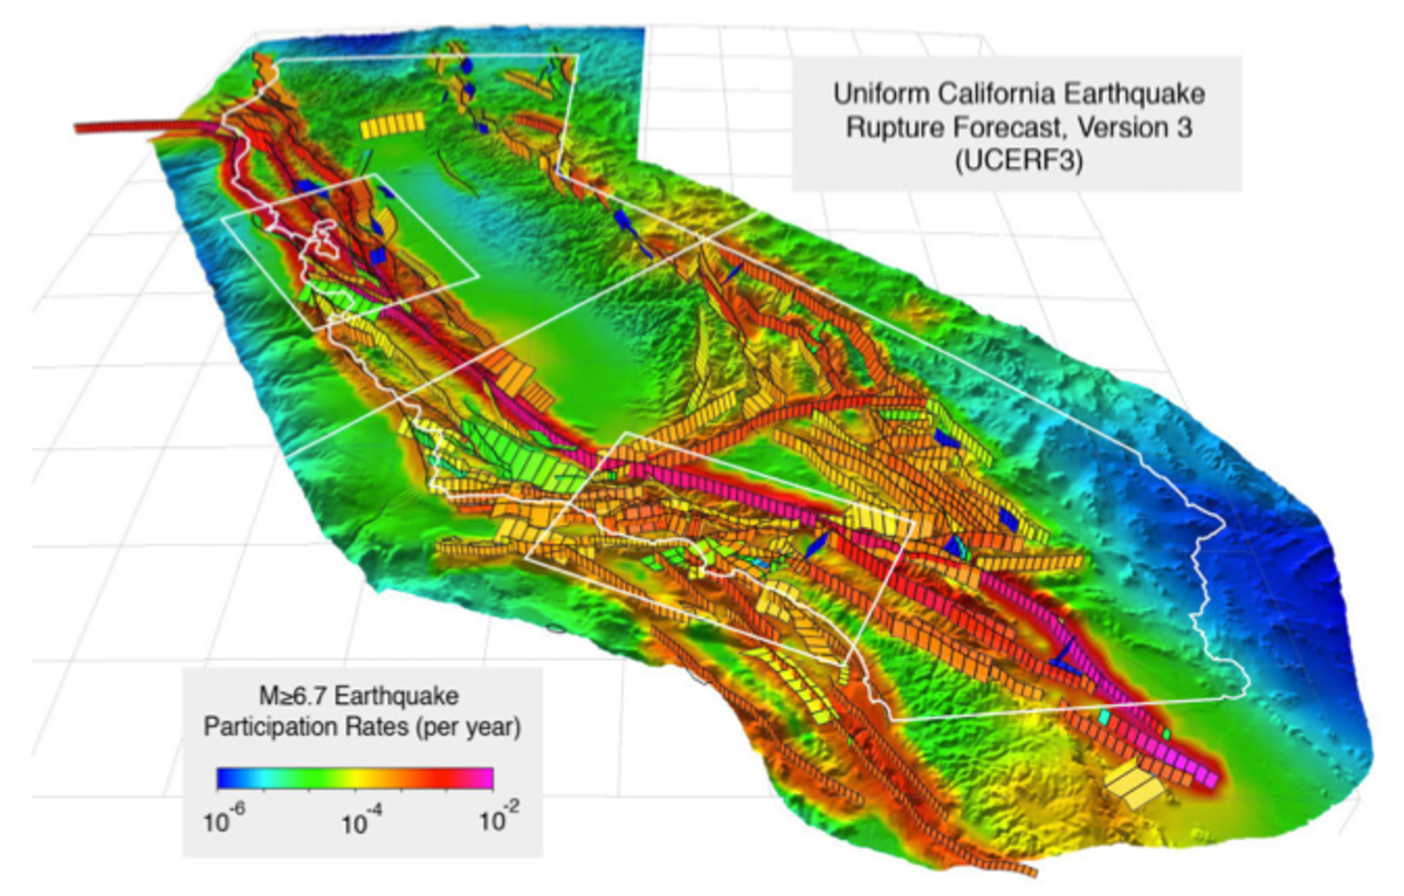
\includegraphics[width=1\textwidth]{img/UCERF3_Map.pdf}
	\end{center}
 \end{columns}	

}

%\decimalpoint
%%%%%%\decimalpoint
%\usepackage{natbib}

%
%\hypersetup{pdfstartview={Fit}, bookmarks=True, pdftitle={SCEC Presentation}, pdfauthor={Juan Carlos Vergara-Gallego}, pdfsubject={Presentation}, pdfkeywords={Waves, Elasticity, Numerical Methods, High Performance Computing, BEM}, pdfpagemode=UseOutlines, bookmarks, bookmarksopen, pdfstartview=FitH, colorlinks,linkcolor=blue, urlcolor=black, citecolor=blue}  % Configure hyperref
%
%%--- New commands ----%
%\newcommand{\footref}[1]{\textsuperscript{\ref{#1}}}
%\newcommand{\pardiff}[2]{\frac{\partial #1}{\partial #2}}
%\newcommand{\pardiffd}[2]{\frac{\partial^2 #1}{\partial #2^2}}
%
%---------------------%
%\usefonttheme[onlymath]{serif}  % Make equations to be in serif fonts
%\usefonttheme{serif}  % Make equations to be in serif fonts

%title


% TITLE PAGE PARAMETERS
%\title{Title}
%\subtitle{~}
%\institute{Institute}
%\author[AUTHOR]{\scriptsize{John Doe$^1$\\Maria Chucena$^2$}\\
%\tiny{$^1$ Doe Industries\\ $^2$ Chucena Inc.}}

\date{\today}


\title[CyberShake] % (optional, only for long titles)
{\justifying CyberShake: A Physics-Based Seismic Hazard Model for Southern California}
%\subtitle{CyberShake, Southern California Earthquake Center}
\author[Vergara, Juan Carlos] % (optional, for multiple authors)
{Juan Carlos Vergara\\ \texttt{\small jvergar2@eafit.edu.co}\\
{\tiny Presentación disponible en: \url{https://github.com/jvergar2/03_SCEC}}}
\institute{Departamento de Ingeniería Civil\\
  Universidad EAFIT}
\date{\today}
\subject{Ingeniería Sísmica}

\begin{document}


% Title page
\begin{frame}[plain]
 \titlepage
\end{frame}
% Outline
%\begin{frame}[allowframebreaks]
%	\frametitle{Contenido}
%	\tableofcontents
%\end{frame}
% OVERVIEW
\begin{frame}[allowframebreaks]
\frametitle{\large{Contenido}}
\begin{enumerate}
\item Introducción
\item Objetivos
\item ¿Qué hacen actualmente?
\item ¿Con qué información cuenta?
	\begin{enumerate}
		\item UCERF $2\.0$ y $3\.0$
		\item Modelos de Velocidad
	\end{enumerate}
\item ¿Qué hacen y como lo hacen?
	\begin{enumerate}
		\item Modelos computacionales
		\item Procesos Ergódicos
		\item Discretización región de estudio
		\item Funciones de Green
		\item Reciprocidad
		\item Tensores de Deformación de Green
	\end{enumerate}
\item Mapas de Amenaza Sísmica
	\begin{enumerate}
		\item Curvas de amenaza
		\item Mapas de Amenaza
	\end{enumerate}
\item Conclusiones
\item Referencias
\end{enumerate}
\end{frame}
%
%
%\section{Introducción}
\begin{frame}
\frametitle{Introducción}
%
\justifying
Se presenta un resumen del proyecto {C}yber{S}hake, de sus objetivos y la foma como están abordando el problema de construir el modelo de Amenaza Sísmica para el Sur de California.

\url{http://scec.usc.edu/scecpedia/CyberShake}
%
\end{frame}
%
%
\begin{frame}[allowframebreaks]
\frametitle{¿Qué es el CyberShake?}
%
\justifying
{C}yber{S}hake, es un proyecto de investigación del ``Southern California Earthquake Center's" (SCEC), dentro del cual se encuentran desarrollando un modelo computacional a gran escala para incluir determinísticamente el efecto de la fuente y la ruta de propagación de las ondas sísmicas en la amenaza sísmica del Sur de California.\\
%
%
%\end{frame}
%\transwipe
%
%\begin{frame}
%\frametitle{¿Qué es el CyberShake?}
\begin{figure}[h]
	\centering
	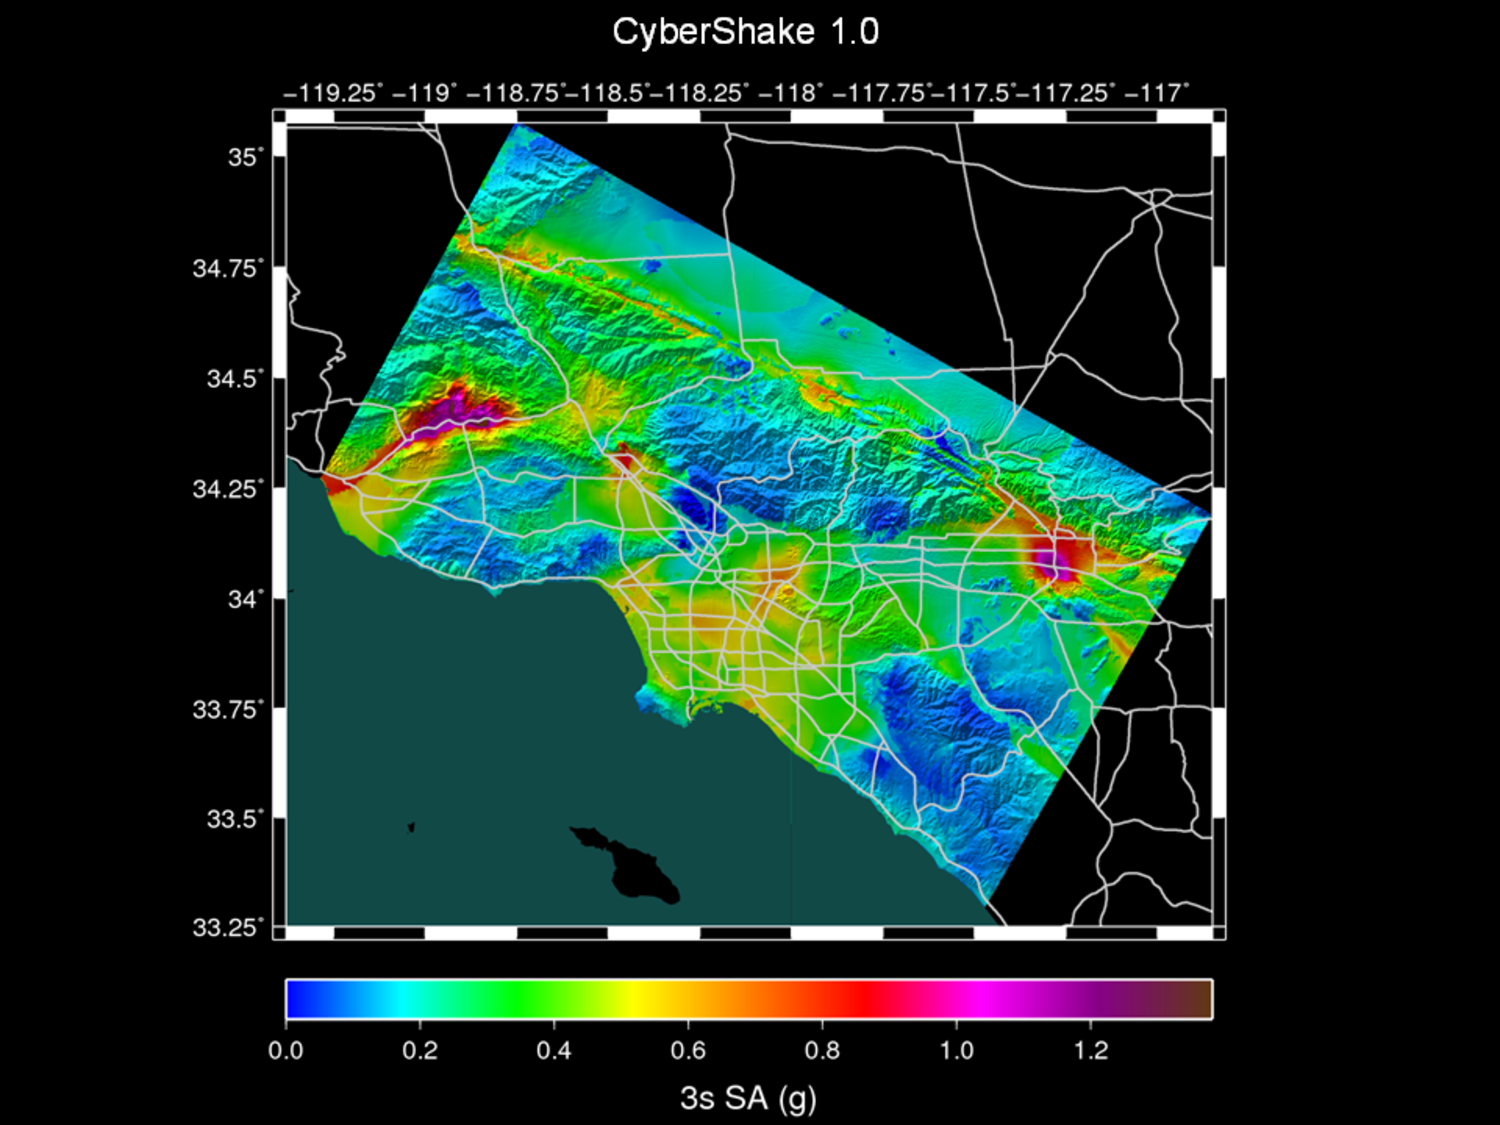
\includegraphics[height=4.5cm]{img/CyberShake_2009.pdf}
	\caption{Mapa de amenaza sísmica del Sur de California calculado con CyberShake. \footnote{\tiny \url{http://scec.usc.edu/scecwiki/images/6/61/CandB_2008.PNG}}}
	\vspace{-.5 cm}
\end{figure} 
%
%\end{frame}
%
%
%\begin{frame}
%\frametitle{¿Qué es el CyberShake?}
%
\begin{figure}[h]
	\centering
	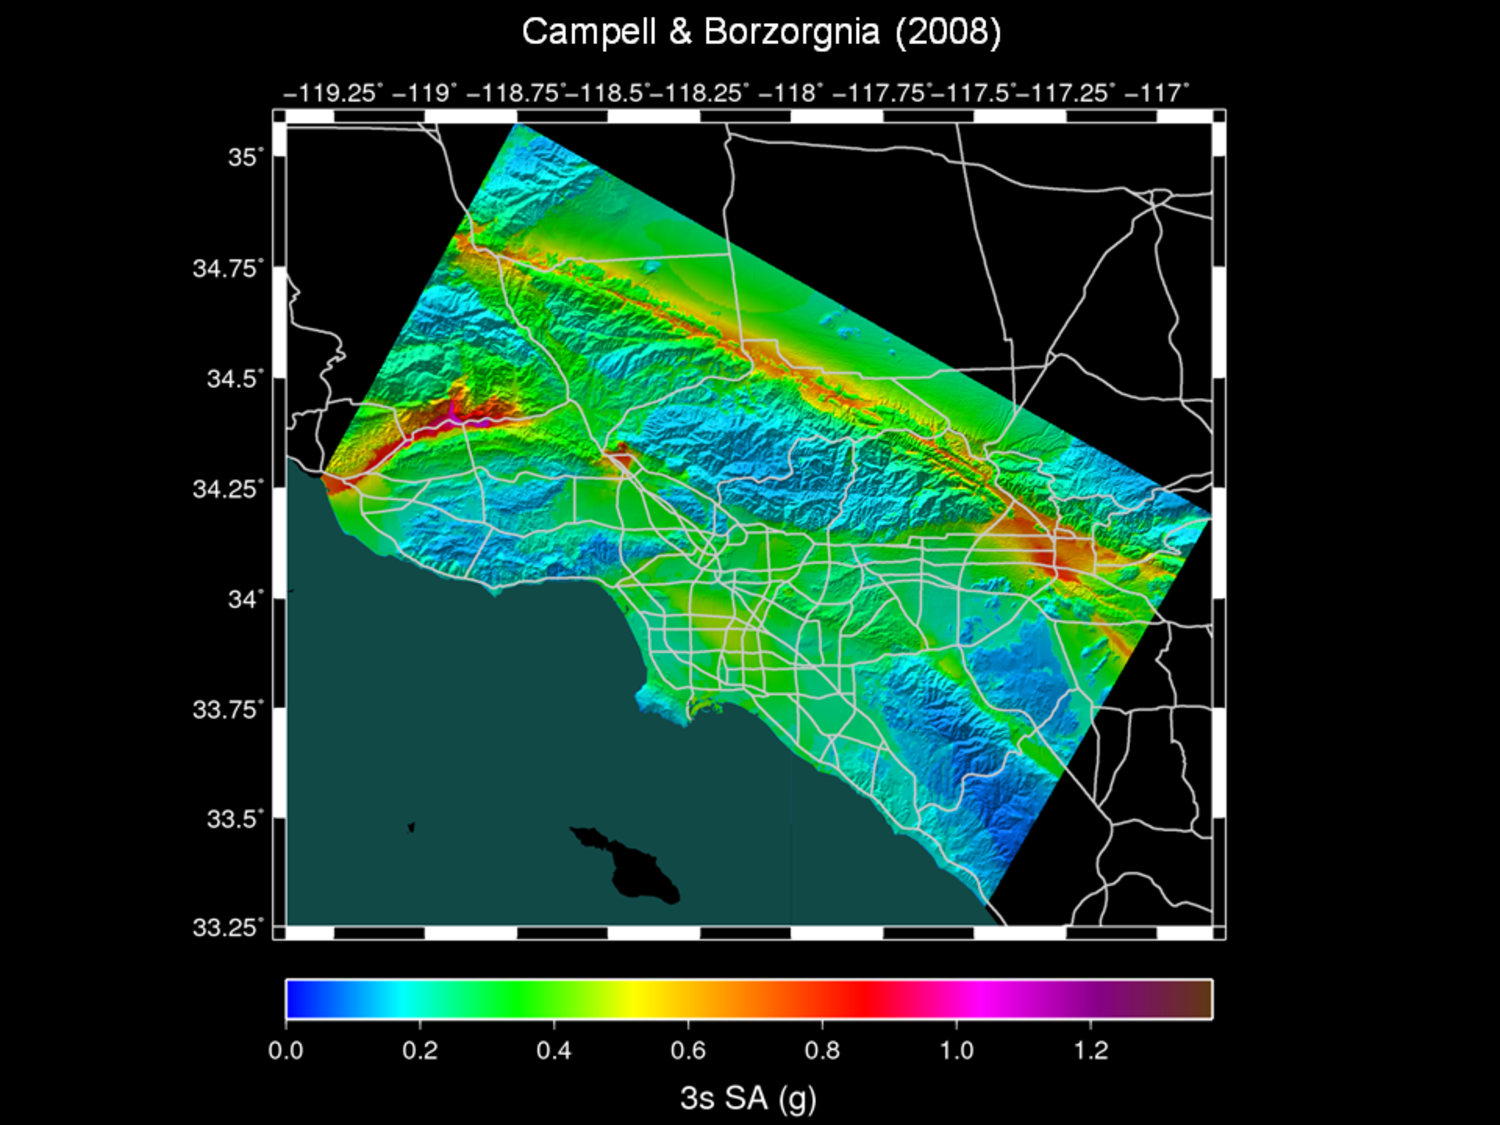
\includegraphics[height=4.5cm]{img/CandB_2008.pdf}
	\caption{Mapa de amenaza sísmica del Sur de California calculado con las ecuaciones de predición del movimiento del suelo (GMPE). \footnote{\tiny \url{http://scec.usc.edu/scecwiki/images/6/61/CandB_2008.PNG}\\}}
	\vspace{-.5 cm}
\end{figure}
%
%
\end{frame}
%
%
%\section{Objetivos}
%\subsection{Objetivos}
\begin{frame}%[allowframebreaks]
\frametitle{Objetivos}
%
\justifying
%
Uno de los objetivos de CyberShake es mejorar las Ecuaciones de Predicción de Movimiento del Suelo (GMPEs), comúnmente usadas en ingeniería.\\
%
El objetivo principal, el objetivo más ambicioso, es remplazar por completo las leyes de atenuación con simulaciones a gran escala para la predicción de los movimientos sísmicos del suelo y con estos calcular los mapas de amenaza sísmica.\\
%
Definir un marco para aplicar la metodología usada en CyberShake en cualquier región del mundo donde se cuente con la información suficiente y se tengan los recursos computacionales.
%
%
\end{frame}
%
%
%\section{¿Qué se hace actualmente?}
\begin{frame}[allowframebreaks]\frametitle{Leyes de Atenuación}
%
\justifying
%
Las Leyes de Atenuación o Ecuaciones de Predicción del Movimiento Sísmico del Suelo (GMPE por sus siglas en Inglés), especifican la probabilidad de excedencia del movimiento del suelo en un sitio particular para una fuente específica representada por un escenario de ruptura específico.\\
%
Las GMPEs entregan $S_a \left( T \right)$ para el $5\%$ de amortiguamiento.\\
%
\begin{figure}[h]
	\centering
	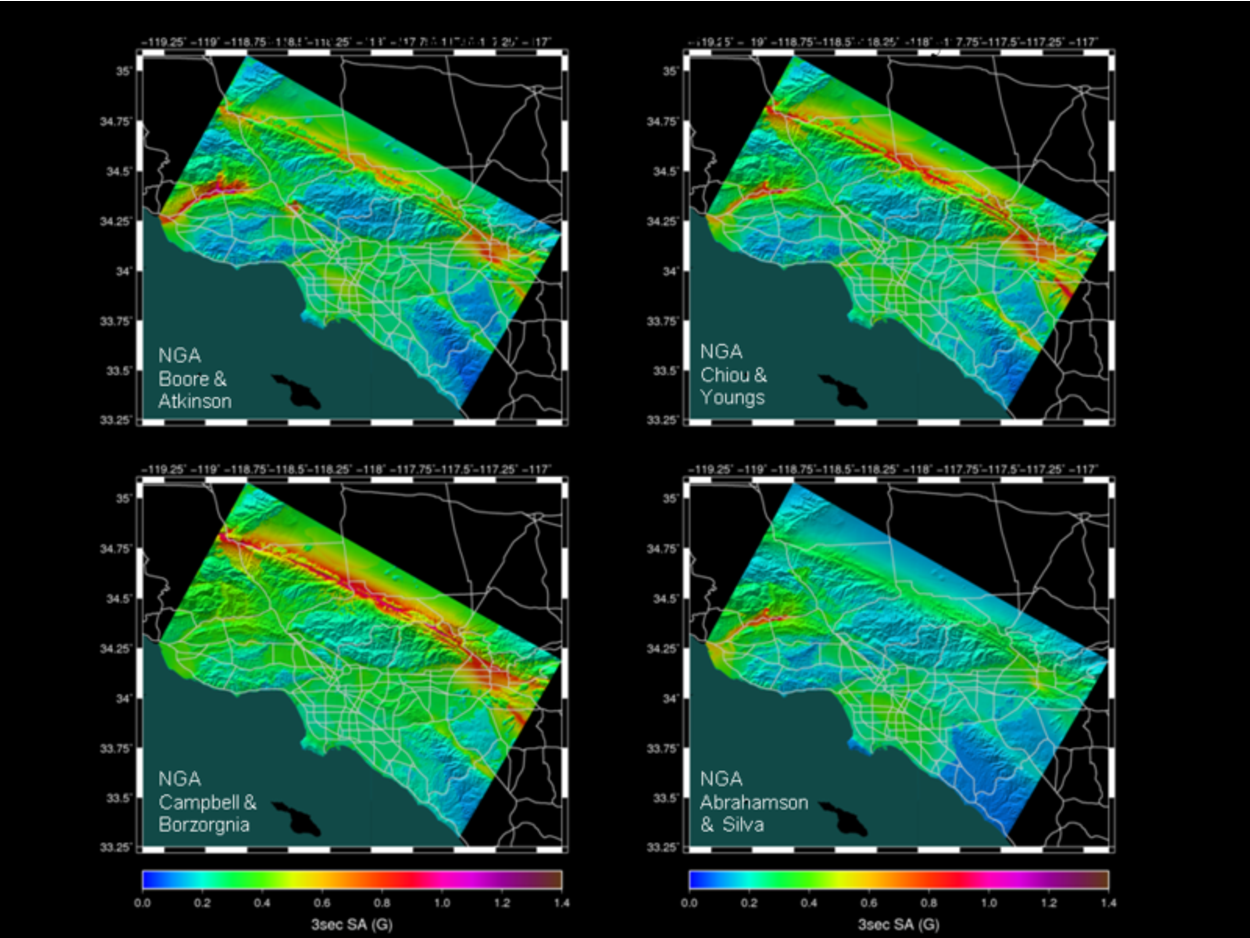
\includegraphics[height=4.5cm]{img/UCERF2_GMPE_2007.pdf}
	\caption{Mapa de amenaza sísmica del Sur de California calculado con cautro ecuaciones de predición del movimiento del suelo (GMPE) diferentes. \footnote{ \tiny\url{http://scec.usc.edu/scecwiki/images/b/bd/UCERF2_GMPE_2007.PNG}\\}}
	\vspace{-.5 cm}
\end{figure}
%
\justifying
%
A pesar de que las cuatro leyes de atenuación son aceptadas en la comunidad científica, es evidente las grandes diferencias entre ellas.\\
%
%
\end{frame}
%
%
%\section{¿Con que información cuentan?}
%\subsection{UCERF $2.0$ y $3.0$}
\begin{frame}[allowframebreaks]
\frametitle{Uniform California Earthquake Rupture Forecast, Version $2\.0$ y $3\.0$}
%
\justifying
%
El $UCERF3\.0$ estima la probabilidad de ocurrencia de sismos, para una magnitud específica y localización, que pueden ocurrir dentro de una ventana de tiempo en California EE.UU. La versión $3\.0$ es una mejora de la versión $2\.0$, dando la posibilidad de la ruptura simultanea de varias fallas y mejorando la sobre-estimación que daba $UCERF2\.0$ para magnitudes entre $6\.5$ y $7\.0$.\\
%
Cuantro componentes básicos de $UCERF3\.0$:
%
	\begin{itemize}
	\justifying
	%
		\item Modelo de Falla: Geometría física de las fallas conocidas.
		%
		\item Modelo de Deformación: ``Tasa de deslizamiento" de cada sección de la falla. Con esto se calcula el momento sísmico.
		%
		\item ``Earthquake Rate Model": Tasa de todos los sismos dentro de una región sobre una magnitud mínima especificada.
		%
		\item Modelos de Probabilidad: Determina la probabilidad de ocurrencia de cada evento dentro de una ventana de tiempo.
	%
	\end{itemize}
%
\begin{figure}[h]
	\centering
	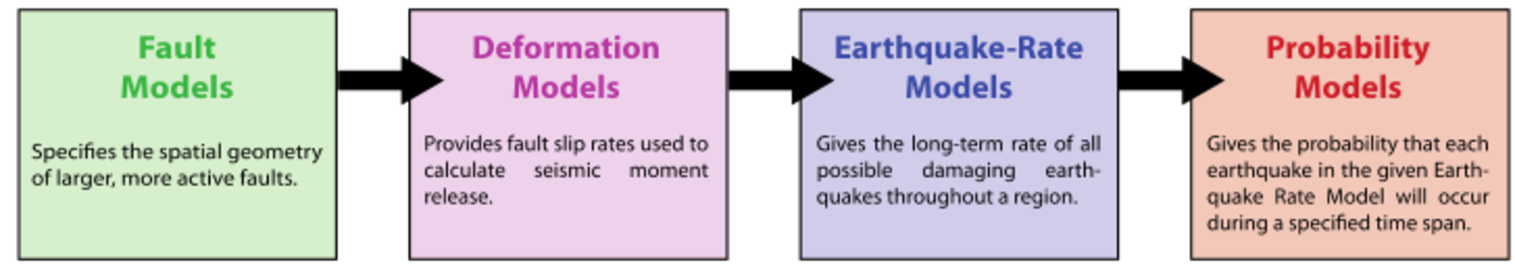
\includegraphics[height=1.75cm]{img/Components_UCERF.pdf}
	\caption{Componentes básicos del modelo UCERF3.0. \cite[figura 2, página 7]{ucerf3}}
\end{figure}
%
%
\justifying
Con la información suministrada por $UCERF2\.0$ se identifican todas las posibles fallas sísmicas $200$ $km$ dentro de la región de estudio. Todas las fallas se usan para generar diferentes escenarios, dentro de los cuales se varía la ubicación del hypocentro y la forma de la ruptura.\\
%
En total se generan al rededor de $415,000$ escenarios de ruptura para cada sitio. 
%
%
%\end{frame}
%%
%%
%\begin{frame}[allowframebreaks]
%\frametitle{Uniform California Earthquake Rupture Forecast, Version $2.0$ y $3.0$ (UCERF $2.0$ y $3.0$)}
%
\begin{figure}[h]
	\centering
	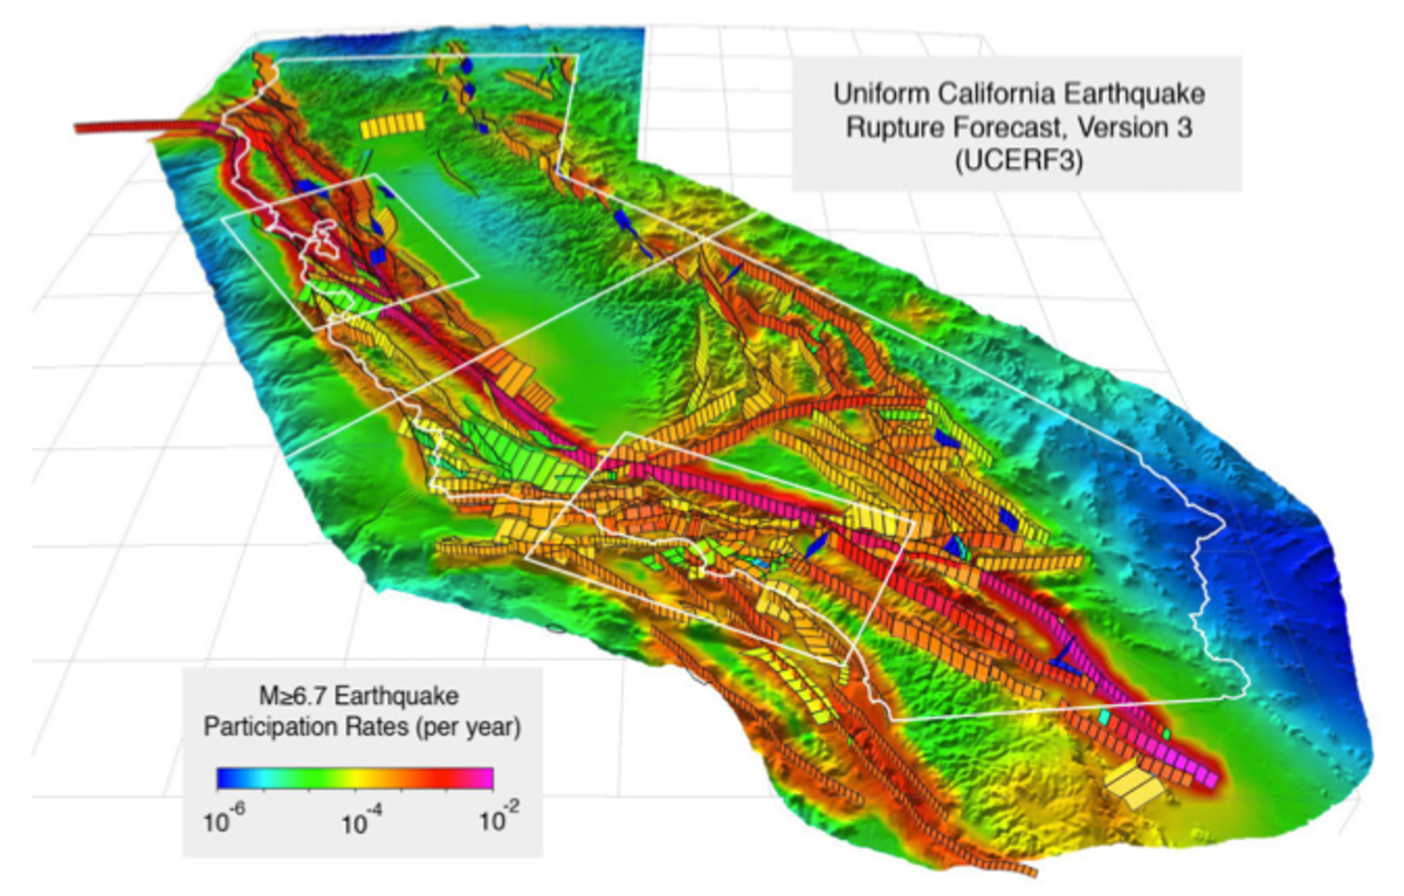
\includegraphics[height=5cm]{img/UCERF3_Map.pdf}
	\caption{Mapa $3D$ de California, mostrando las $2606$ fallas mapeadas en $UCERF3\.0$ \cite[figura 1, página 5]{ucerf3}}
\end{figure}
%
\end{frame}
%
%
%\subsection{Modelos de Velocidad}
\begin{frame}[allowframebreaks]
\frametitle{SCEC Community Velocity Model: CVM-S.}
%
\justifying
%
El modelo de velocidad comunitario de California (CVM-S \footnote{ \tiny Actualmente se encuentra disponible en linea la versión $4\.0$ de dicho modelo. \url{http://www.data.scec.org/research-tools/3d-velocity.html}, \url{http://scec.usc.edu/scecpedia/CVM-S}, último acceso $03$ de Octubre de $2014$.}, por sus siglas en ingles), tiene como propósito servir como modelo de referencia en varias áreas de investigación que dependen de las estrucutras, propiedades de los materiales tales como la velocidad de propagación de las ondas sísmicas, en profundidad para llevar acabo diferentes análisis. Las velocidades de mayor profundidad se construye con base reglas que relacionan la profundidad y la edad de los depósitos sedimentarios con las velocidades de las ondas sísmicas. Las velocidades de propagación en los depósitos menos profundos son tomadas de las medidas de los estudios geotécnicos. Las velocidades de propagación en roca son tomados de estudios tomográficos.\\
%
El modelo de velocidad CVM-S es de libre acceso, un usuario puede obtener los códigos escritos en Fortran, compilarlos y ejecutarlos en una máquina personal. El código se alimenta con un archivo de texto que contiene la latitud, longitud y profundidad de puntos donde se quiere conocer $V_p$, $V_s$ y $\rho$.
%
%
\begin{figure}[h]
	\centering
	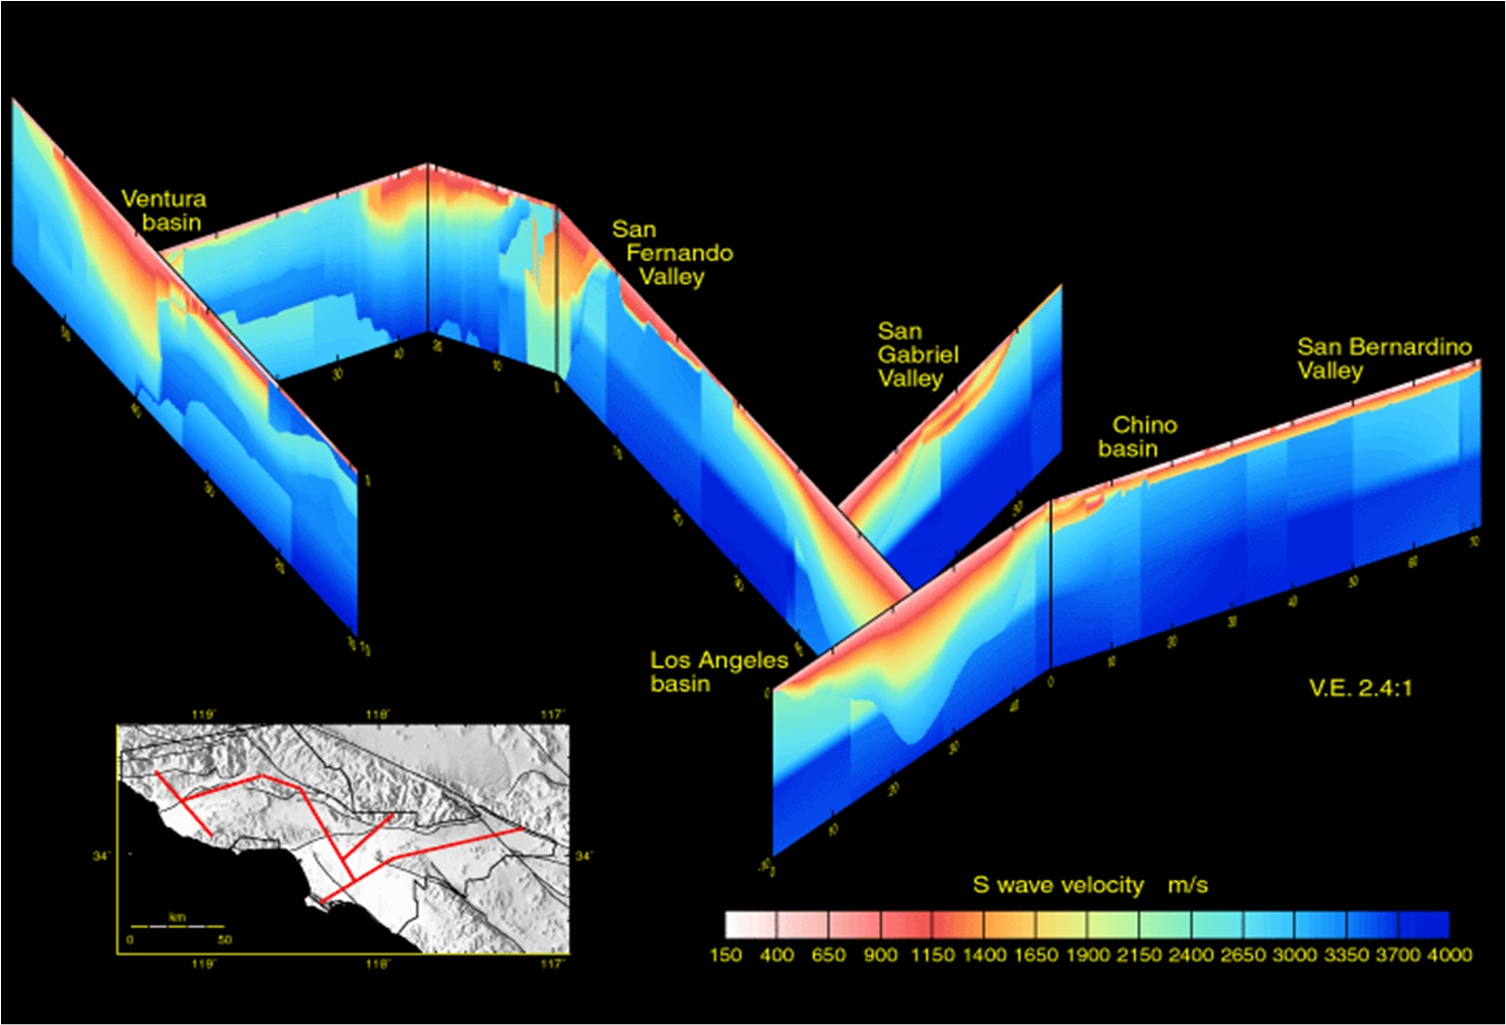
\includegraphics[height=4.5cm]{img/CVM-S4.pdf}
	\caption{Secciones transversales de California mostrando la variación en profundidad de la velocidad. \footnote{\tiny \url{http://scec.usc.edu/scecwiki/images/a/a7/CVM-S4.png}\\}}
	\vspace{-.5 cm}
\end{figure}
%
\end{frame}
%
%
\begin{frame}[allowframebreaks]
\frametitle{SCEC Community Velocity Model: CVM-H.}
%
\justifying
%
El Modelo de Velocidad Comunitario - Harvard (CVM-H \footnote{\tiny Actualmente se encuentra disponible en linea la versión $11\.9\.0$ de dicho modelo. \url{http://scec.usc.edu/scecpedia/CVM-H}}, por sus siglas en ingles), se basa en ensayos de reflexión sísmica y ``Borehole" para la estimación de la velocidad de propagación de la onda sísmica en puntos específicos. Dicha información se interpola en una malla bastante refinada cubriendo toda la región que se quiere estudiar. Adicionalmente contiene una descripción extensiva del modelo de velocidad en la región fuera de la costa (offshore).
%
\begin{figure}[h]
	\centering
	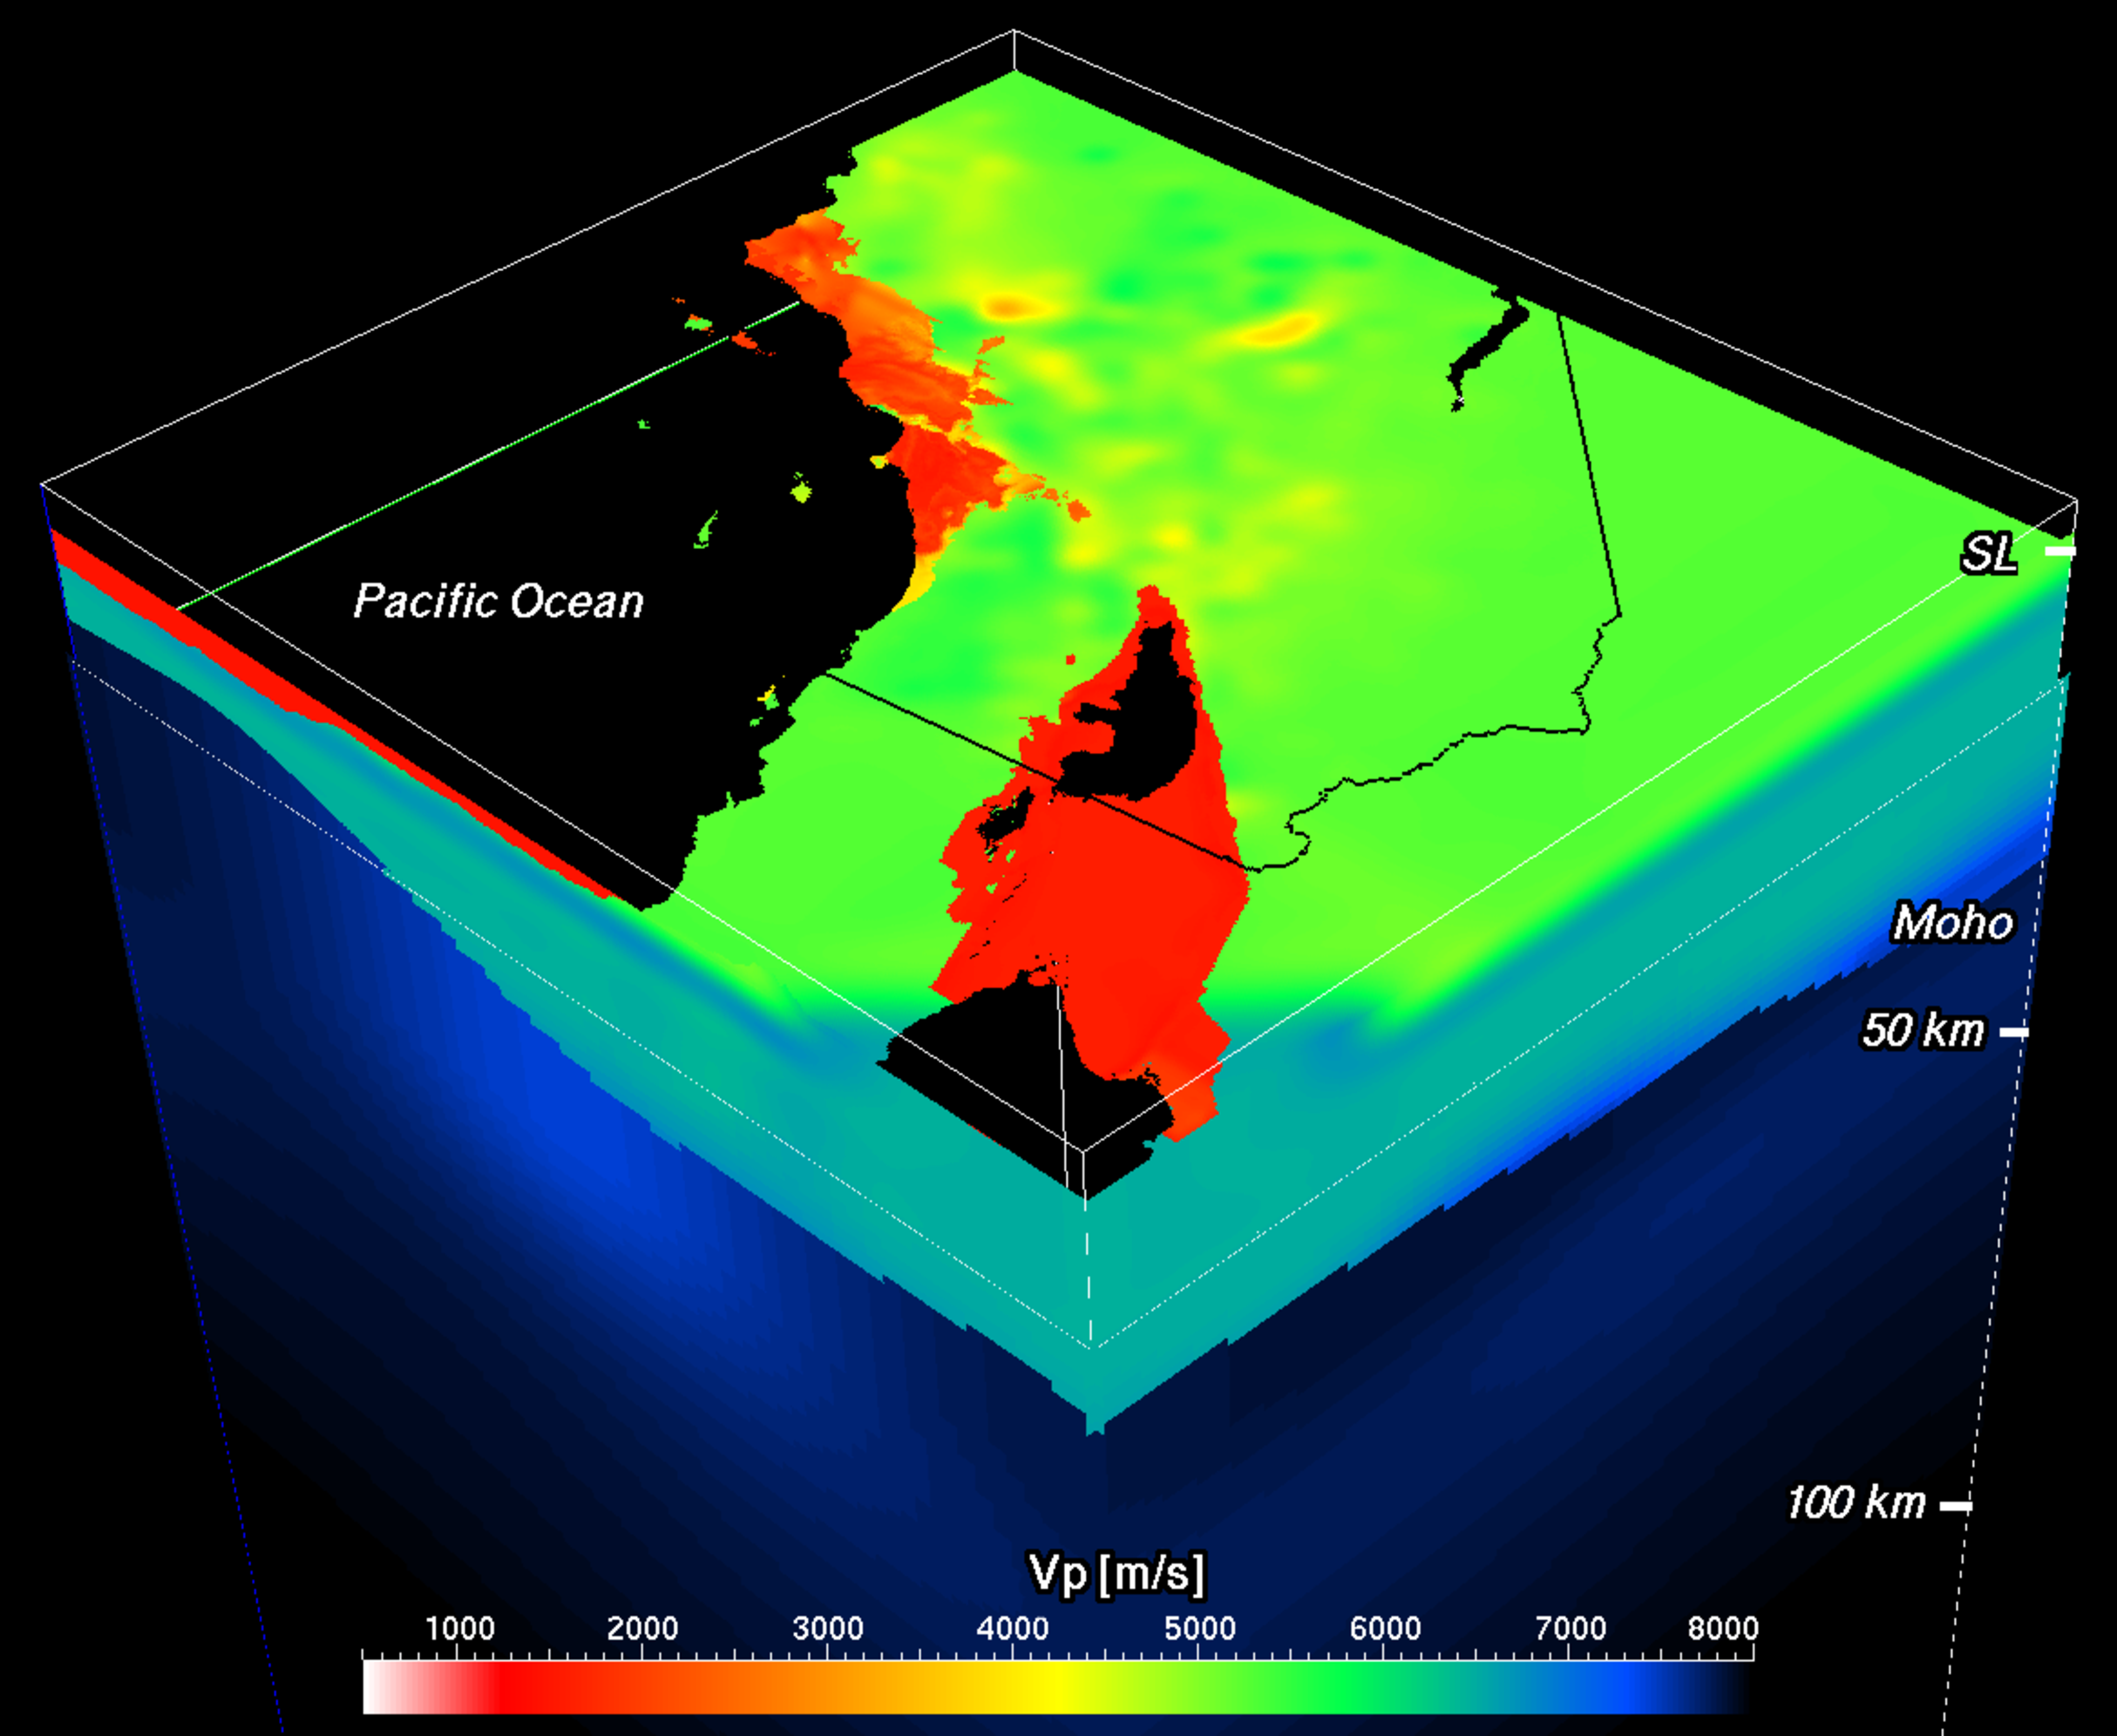
\includegraphics[height=4.5cm]{img/CVM64_perspectve.pdf}
	\caption{Perspectiva Modelo de Velocidad Comunitario - Harvard (CVM-H). \footnote{\tiny\url{http://scec.usc.edu/scecwiki/images/a/a1/CVM64_perspectve.png}\\}}
	\vspace{-.5 cm}
\end{figure}
%
%
\end{frame}
%
%
%\section{¿Qué hacen y cómo lo hacen?}
%\subsection{Modelos Computacionales}
\begin{frame}%[allowframebreaks]
\frametitle{Modelos computacionales}
%
\justifying
%
En un sitio particular, es necesario conocer la incidencia de varios eventos sísmicos, generados por diferentes sismofuentes, para poder generar unas curvas de amenaza sísmica lo suficientemente confiables.\\
%
Teniendo los modelos computacionales a gran escala, es posible generar cuantos eventos sísmicos sean necesarios y tener en cuenta la generación de sismos desde varios tipos de fuentes, tener en cuenta la incidencia de los factores tales como la ruta de propagación de las ondas, los efectos de fuente y sismos de diferentes magnitudes generados por una misma fuente.\\
%
En un sitio particular, CyberShake directamente muestrea la variabilidad del movimiento del suelo a partir de información de varios sismos (escenarios de ruptura) y elimina la necesidad de asumir que los procesos son ergódicos.
%
\end{frame}
%
%
%\subsection{Procesos Ergódicos}
\begin{frame}%[allowframebreaks]
\frametitle{Procesos Ergódicos}
%
\justifying
%
\begin{figure}[h]
	\centering
	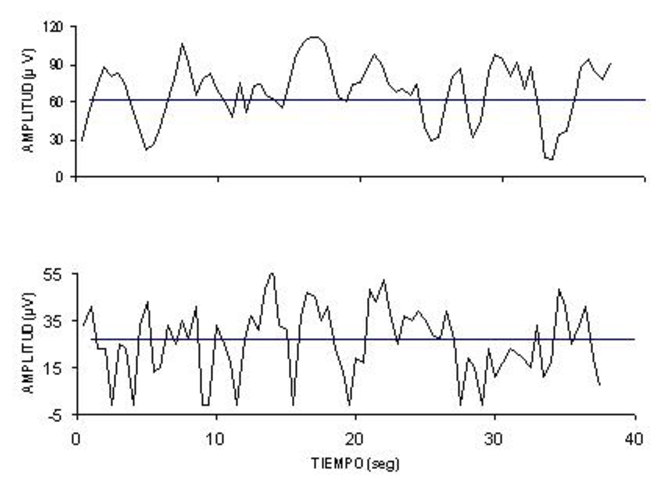
\includegraphics[height=3cm]{img/Ergodico.pdf}
	\caption{Definición gráfica de un proceso Ergódico. Imagen tomada de \footnote{\tiny \url{http://www.iga.cu/publicaciones/revista/cte_07/art_07-01/id28.htm}\\}}
	\vspace{-.5 cm}
\end{figure}
%
\textbf{Proceso Ergódico:} Los promedios o medias hacia la derecha son iguales hacia abajo. Es lo mismo hallar los indicadores de un acelerograma que de varios.\\
%
\end{frame}
%
%
%\subsection{Discretización región de estudio}
\begin{frame}[allowframebreaks]
\frametitle{Discretización de la región de estudio}
%
\justifying
\begin{figure}[h]
	\centering
	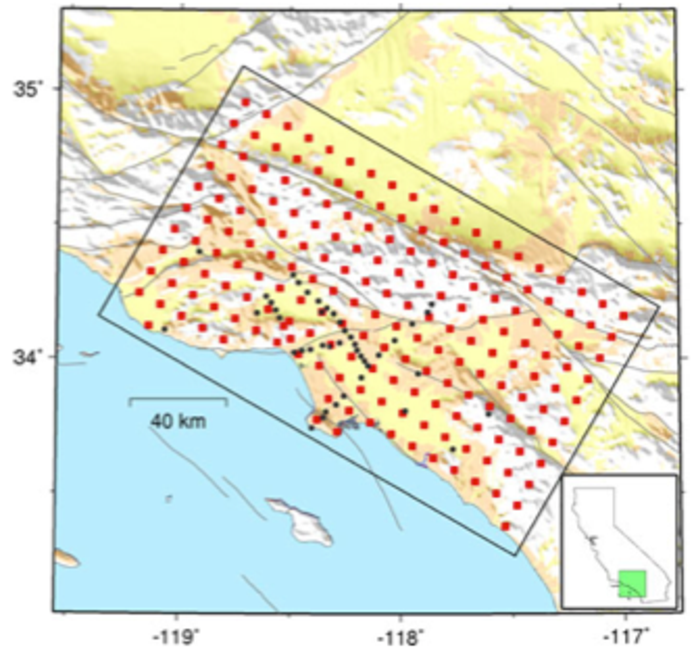
\includegraphics[height=4.5cm]{img/Discretizacion.pdf}
	\caption{Mapa del Sur de California mostrando los puntos en los cuales se calculan las curvas de amenaza. \cite[figura 1, página 3]{gravesetal}}
	\vspace{-.5 cm}
\end{figure}
%
Dentro del proyecto CyberShake, se han simulado diferentes escenarios de ruptura y se han calculado las curvas de amenaza en $250$ sitios en la región de Los Angeles, con lo cual tienen las bases para la generación de mapas de amenaza sísmica a partir de CyberShake.\\
%
%
\end{frame}
%
%
\begin{frame}[allowframebreaks]
\frametitle{¿Por qué no calcular las curvas de amenaza en los puntos de la malla en superficie?}
%
\justifying
%
Dentro de la región de Los Angeles se tienen identificadas al rededor de $10,000$ fallas que pueden generar sismos de intensidad mayor igual a $6\.0$ $(M_w \geq 6\.0)$ que pueden afectar la región bajo estudio.
%
\begin{figure}[h]
	\centering
	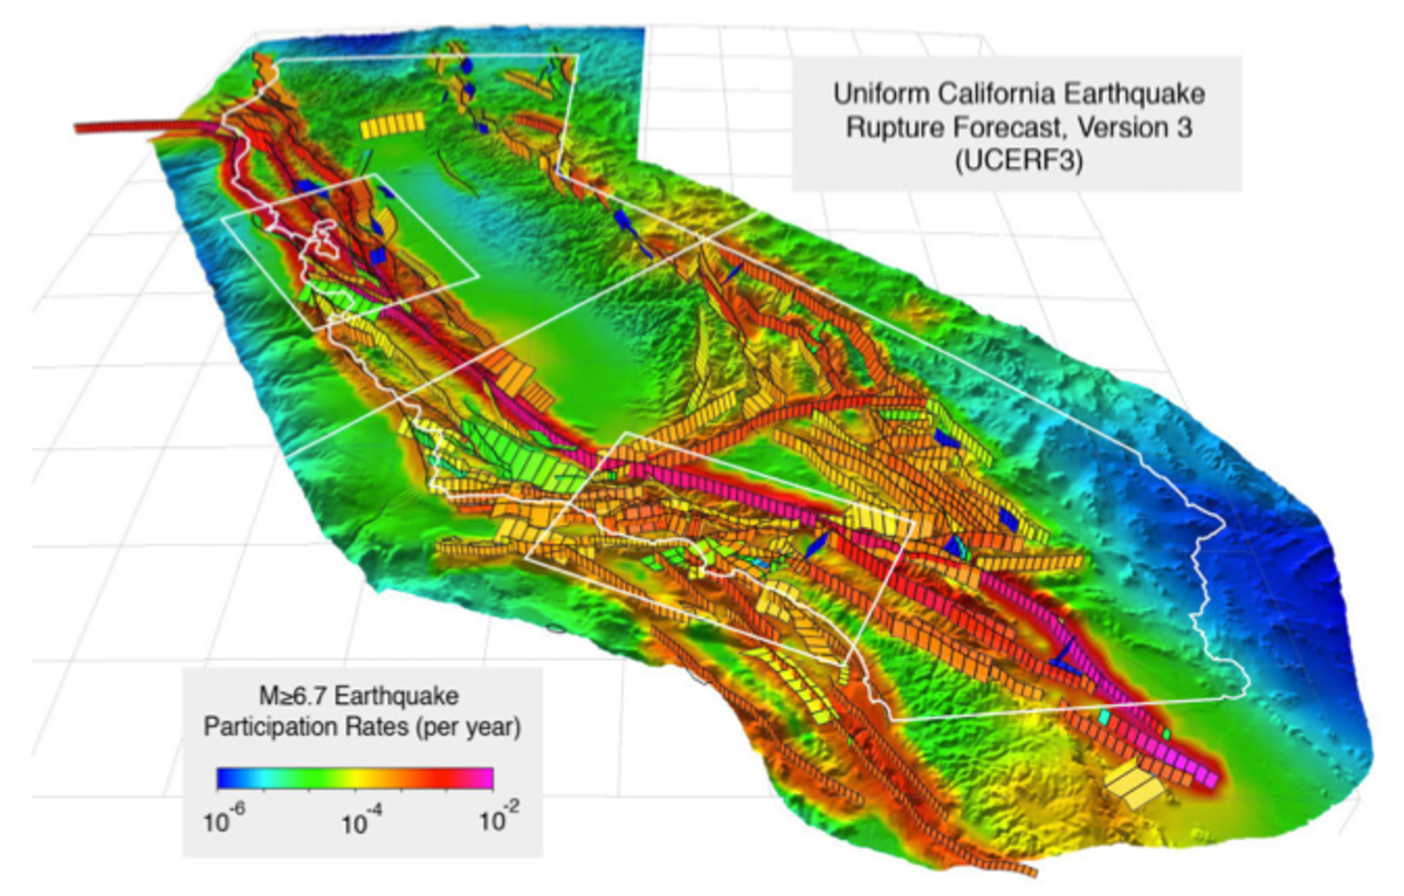
\includegraphics[height=4.5cm]{img/UCERF3_Map.pdf}
	\caption{Mapa $3D$ de California, mostrando las $10,000$ fallas mapeadas en $UCERF3\.0$ \cite[figura 1, página 5]{ucerf3}}
\end{figure}
%
A partir de cada falla se generan diferentes escenarios, donde se varían factores tales como la ubicación del hipocentro, magnitud del evento y proceso de ruptura. Dentro de CyberShake se han generado al rededor de $415,000$ escenarios diferentes.\\
%
\begin{figure}[h]
	\centering
	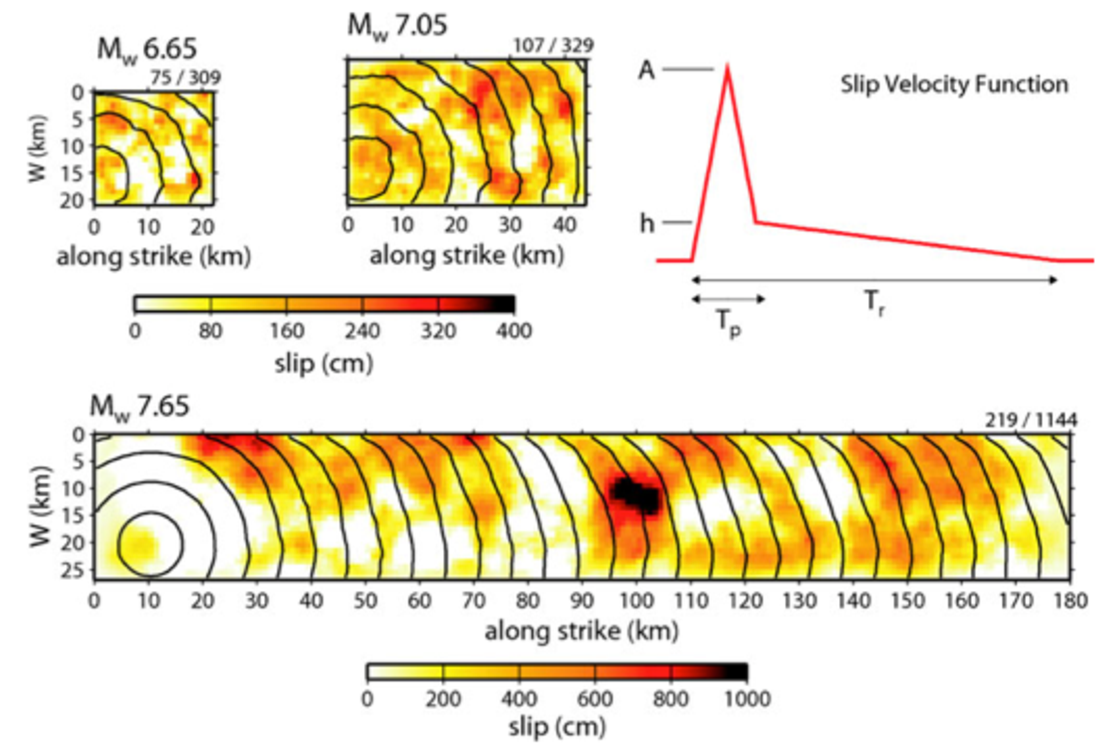
\includegraphics[height=4.5cm]{img/ModeloRuptura.pdf}
	\caption{Cinemática para diferentes escenarios de ruptura. \cite[figura 4, página 7]{gravesetal}}
\end{figure}
%
Cada escenario diferente representa un modelo computacional diferente, por lo cual sería necesario analizar $415,000$ modelos $3D$ a gran escala con los costos computacionales que esto representa y la cantidad de información que se genera.\\ 
%
%
\end{frame}
%
%
%\subsection{Funciones de Green}
\begin{frame}[allowframebreaks]
\frametitle{Funciones de Green en Elastodinámica}
%
\justifying
%
\textbf{Función de Green en Elastodinámica:} Desplazamiento debido a una fuente puntual.
%
\begin{figure}[h]
	\centering
	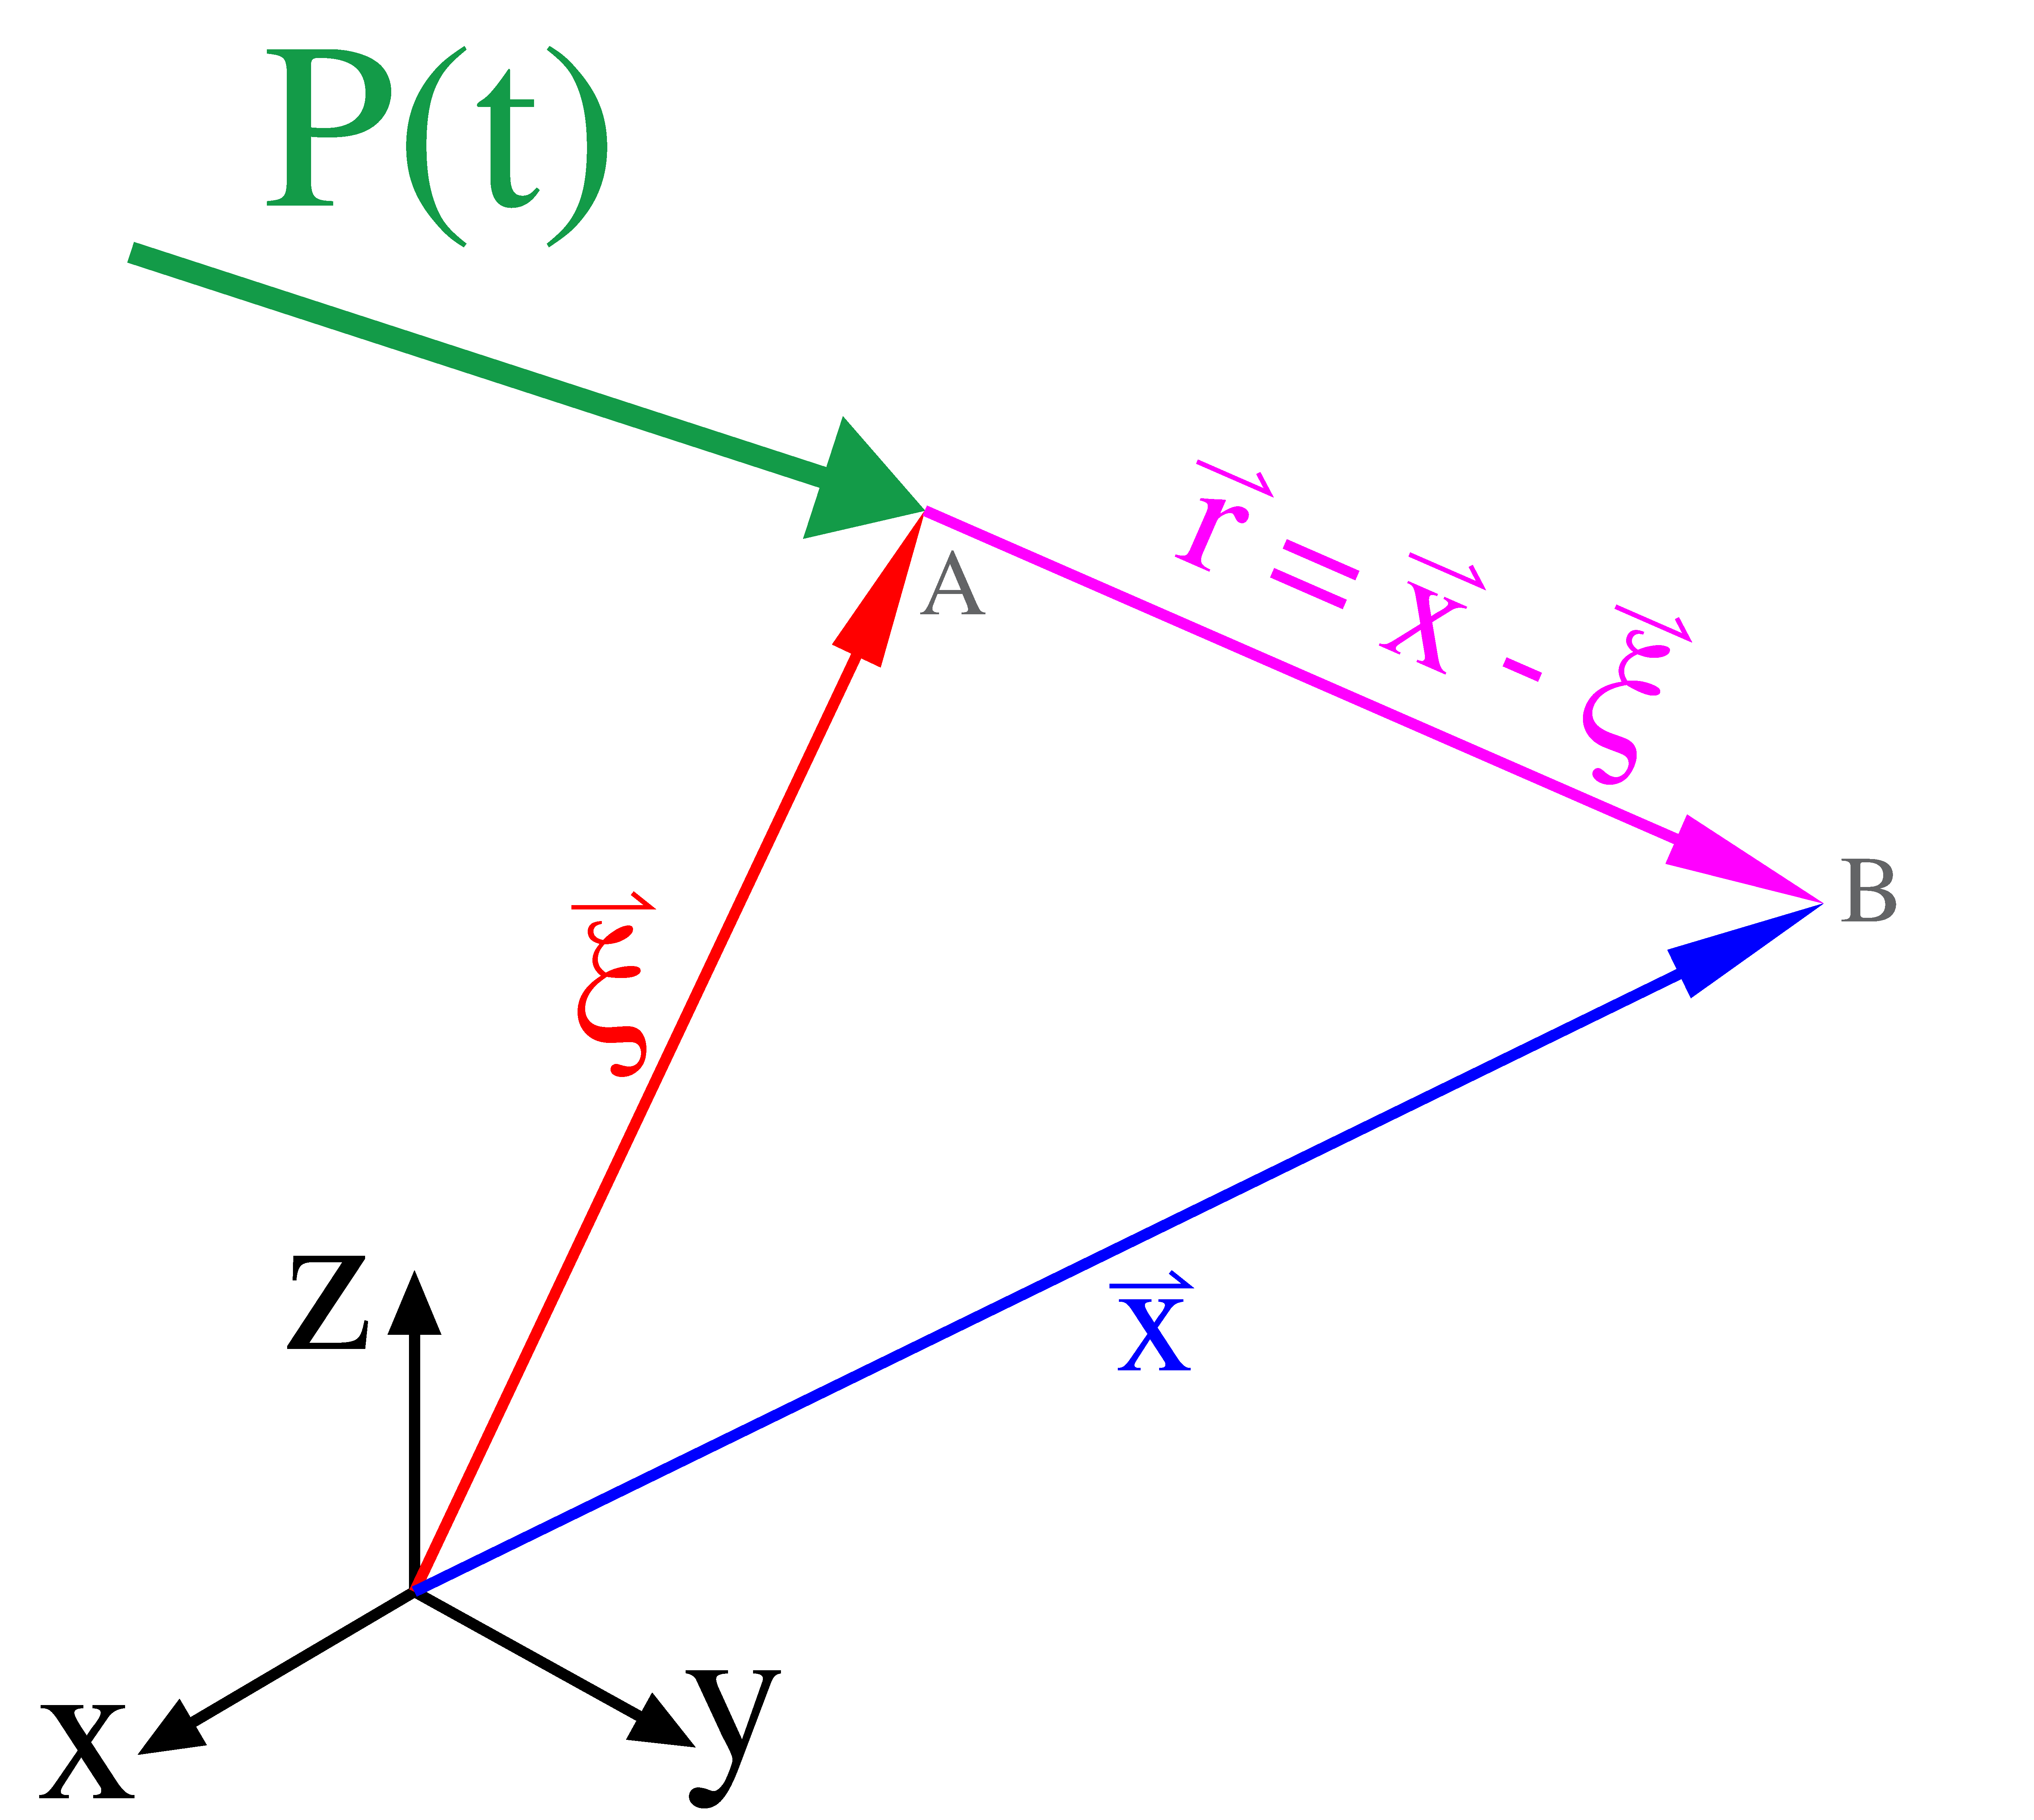
\includegraphics[height=4.5cm]{img/Figure1.pdf}
	\caption{Nomenclatura Función de Green.}
	\vspace{-.5 cm}
\end{figure}
%
\begin{align*}
	\mathbf{G}_{in} \left( \vec{x}, t; \vec{\xi}, \tau \right) \text{Función de Green}\\
\end{align*}
%
Donde:
%
\begin{itemize}
%
	\item $\vec{x}:$ Ubicación en la cual se quiere conocer el desplazamiento.
	%
	\item $t:$ Tiempo en el cual se desea cononcer el desplazamiento en el punto $\vec{x}$.
	%
	\item $\vec{\xi}:$ Punto de aplicación de la carga puntual.
	%
	\item $\tau:$ Tiempo en el cual se aplica la carga en el punto $\vec{\xi}$.
%
\end{itemize}
%
%
\end{frame}
%
%
%\subsection{Reciprocidad}
\begin{frame}[allowframebreaks]
\frametitle{Reciprocidad en Elastodinámica}
%
\justifying
%
Sobre un punto $\vec{\xi}_1$ de un medio continuo actúa una carga $\vec{f}_m$ en dirección $\hat{m}$ y sobre un punto $\vec{\xi}_2$ actúa una carga $\vec{g}_n$ en dirección $\hat{n}$.
%
%\begin{figure}[h]
%\centering
%%
%	\subfloat[Carga 1]{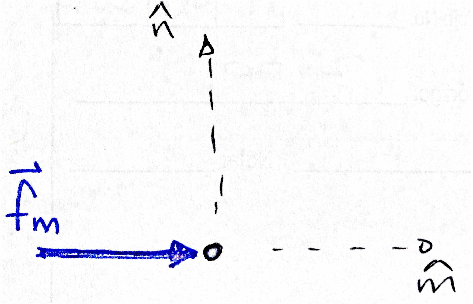
\includegraphics[width=0.35\textwidth]{img/Recipro1.pdf}}
%	%
%	\subfloat[Carga 2]{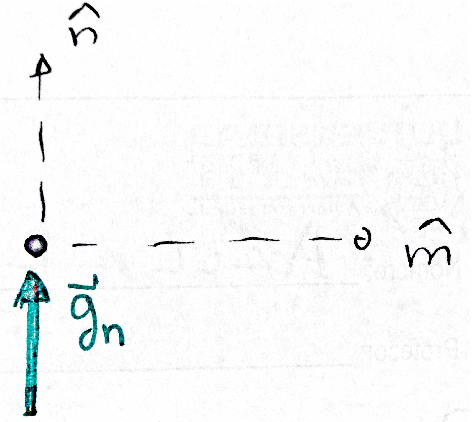
\includegraphics[width=0.35\textwidth]{img/Recipro2.pdf}}
%	%
%	\caption{Reciprocidad}
%	\vspace{-.5 cm}
%%
%\end{figure}
%
\begin{figure}[h]
	\centering
	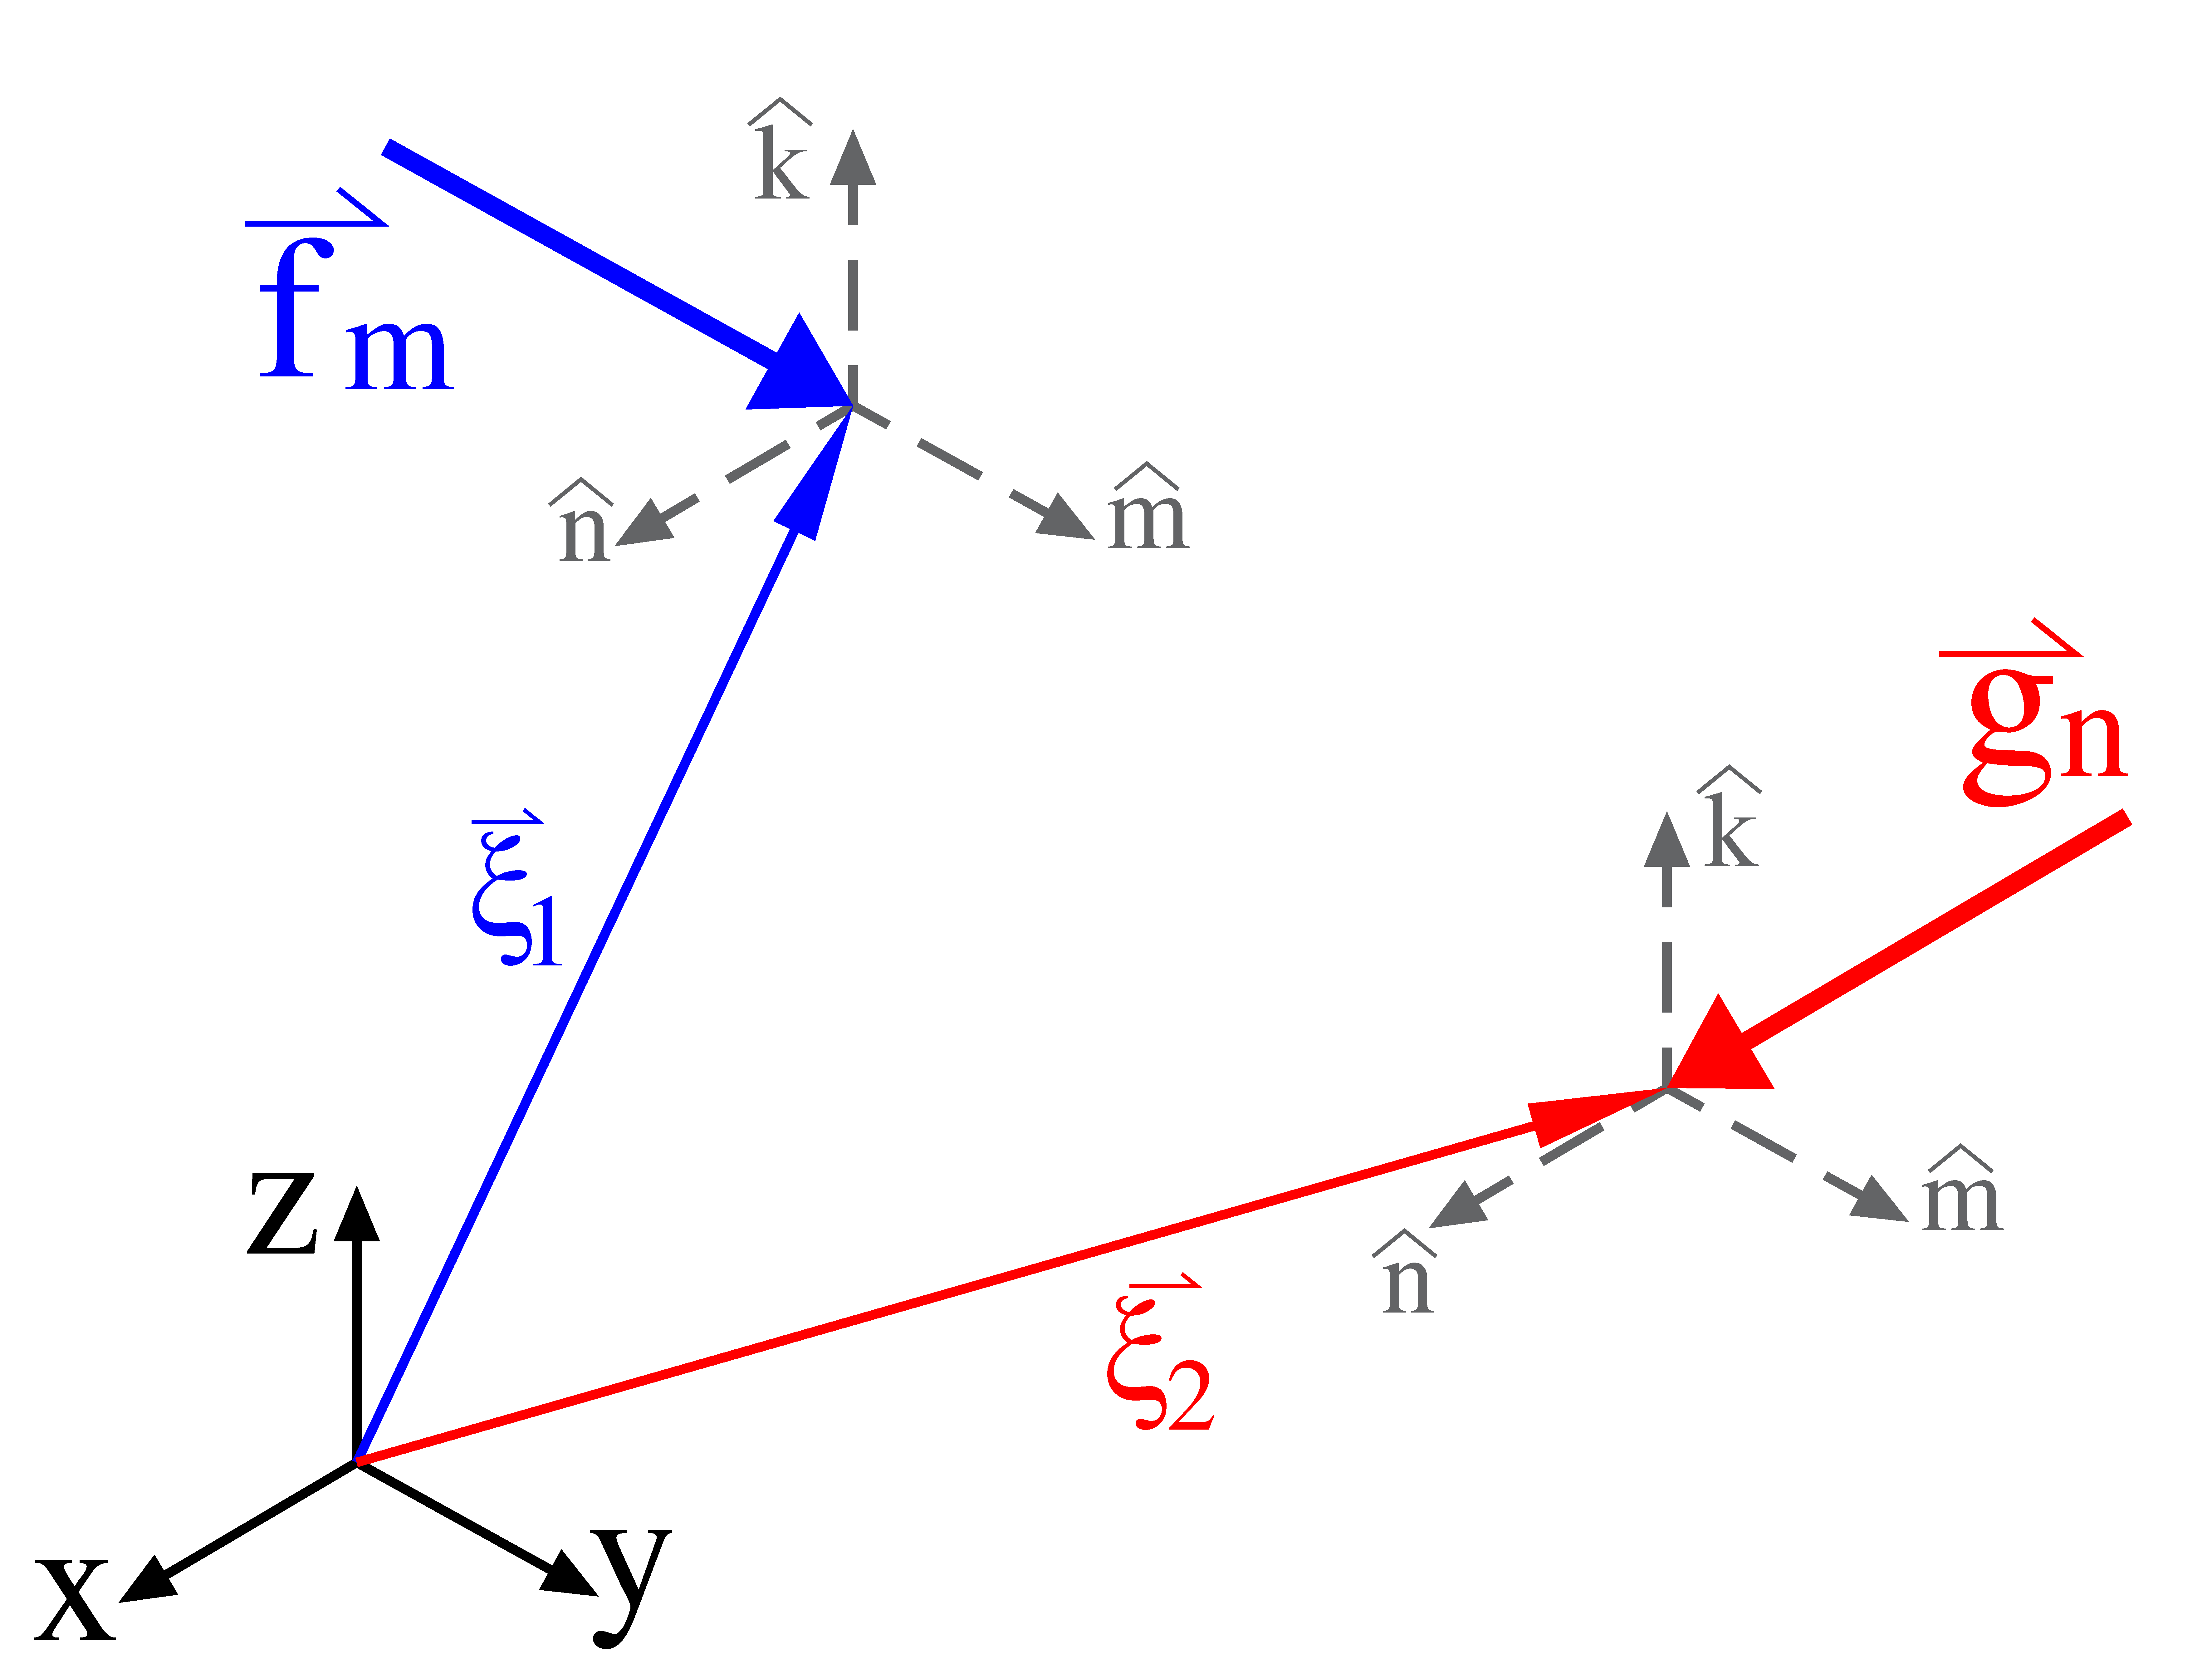
\includegraphics[height=4cm]{img/Reciprocity.pdf}
	\caption{Reciprocidad}
	\vspace{-.5 cm}
\end{figure}
%
Si $\vec{f}_m$ y $\vec{g}_m$ son fuerzas unitarias, se puede afirmar que:\\
%
El desplazamiento que se genera en el punto $\vec{\xi}_2$ en la dirección $\hat{n}$ debido a la aplicación de una carga unitaria en $\vec{\xi}_1$ en la dirección $\hat{m}$, es igual al desplazamiento que se genera en el punto $\vec{\xi}_1$ en la dirección $\hat{m}$ si la carga unitaria se aplica en el punto $\vec{\xi}_2$ en la dirección $\hat{n}$.
%
\begin{align*}
	\mathbf{G}_{nm} \left( \vec{\xi}_2, \tau ; \vec{\xi}_1, 0 \right)  = \mathbf{G}_{mn} \left( \vec{\xi}_1, \tau ; \vec{\xi}_2, 0 \right) \hspace{1 cm} \textbf{donde: $\tau_1=\tau_2=0$}\\
	%
	\mathbf{G}_{nm} \left( \vec{\xi}_2, \tau_2 ; \vec{\xi}_1, \tau_1 \right)  = \mathbf{G}_{mn} \left( \vec{\xi}_1, -\tau_1 ; \vec{\xi}_2, -\tau_2 \right) \hspace{1 cm} \textbf{donde: $\tau=0$}
\end{align*}
%
Donde las ecuaciones anteriores representan la reciprocidad espacial y espacio-temporal respectivamente.
%
%
\end{frame}
%
%
%\subsection{Tensores de Deformación de Green}
\begin{frame}[allowframebreaks]
\frametitle{¿Cómo se calculan las SGT?}
%
\justifying
%
CyberShake discretiza la región de estudio en $250$ sitios en los cuales se quiere calcular la curva de amenaza, puntos en los cuales se quieren conocer los registros sintéticos.
%
\begin{figure}[h]
	\centering
	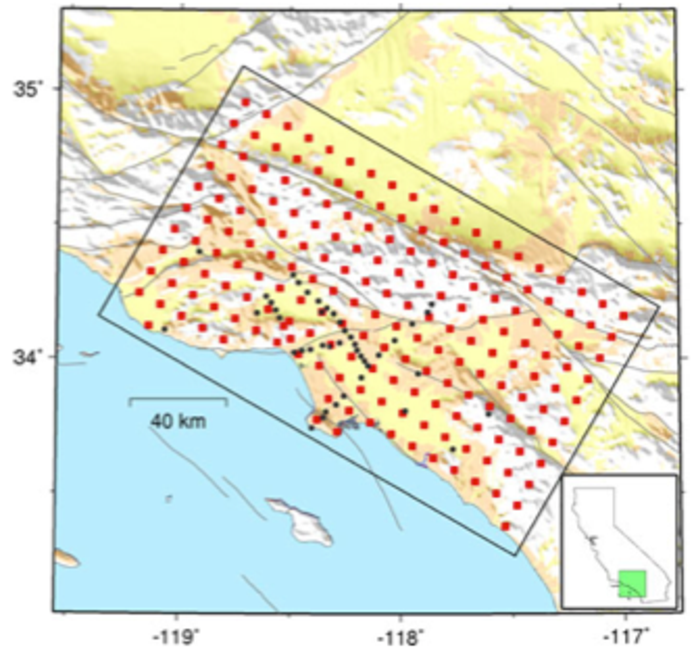
\includegraphics[height=3cm]{img/Discretizacion.pdf}
	\caption{Mapa del Sur de California mostrando los puntos en los cuales se calculan los registros sintéticos. \cite[figura 1, página 3]{gravesetal}}
	\vspace{-.5 cm}
\end{figure}
%
%
\begin{figure}[h]
	\centering
	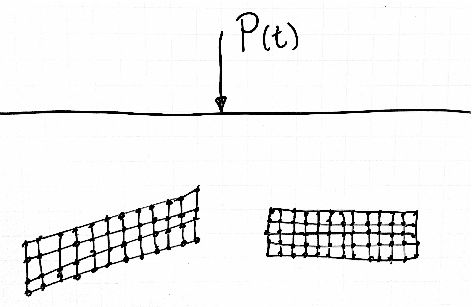
\includegraphics[height=6cm]{img/SGT.pdf}
	\caption{Cálculo de la funciones de Green}
	\vspace{-.5 cm}
\end{figure}
%
%
En cada uno de los $250$ puntos en los que se discretiza la región se aplica un carga unitaria en dos direcciones ortongales, cada carga aplicada es un análisis independiente y no se aplica la componente vertical pues dentro de CyberShake no están interesados en esta componente, y se calculan los tensores de deformación de Green sobre los puntos en los cuales se tienen discretizadas todas las fallas para cada una de las cargas.\\
%
Gradiente de Espacial de Deformación:
%
\begin{align*}
	\varepsilon \left( \vec{r}, t \right) = \dfrac{1}{2} \left\lbrace \left[ \mathbf{\nabla u } \left( \vec{r}, t \right) \right] + \left[ \mathbf{\nabla u} \left( \vec{r}, t \right) \right]^T \right\rbrace
\end{align*}
%
Es posible conocer el tensor de deformación de orden $3$, de forma análoga al Gradiente de Deformación Espacial, usando el gradiente espacial de los elementos del Tensor de green:
%
\begin{align*}
	\mathbf{H} \left( \vec{r}, t;\vec{r}_s \right) = \dfrac{1}{2} \left\lbrace \left[ \mathbf{\nabla G} \left(\vec{r}, t; \vec{r}_s \right) \right] + \left[ \mathbf{\nabla G} \left( \vec{r}, t; \vec{r}_s \right) \right]^{213} \right\rbrace
\end{align*}
%
Donde:
%
\begin{itemize}
%
	\justifying
	\item $\vec{r}_s:$ Ubicación donde se aplica la carga de Green, el gradiente espacial opera sobre $\vec{r}$.
	%
	\item $\left[  \cdot \right]^{213}:$ Indica transposición en los dos primeros índices del tensor.
%
\end{itemize}
%
En notación indicial:
%
\begin{align*}
\left[ \mathbf{H}_{inj} \right]^{213} = \mathbf{H}_{nij}
\end{align*}
%
\begin{align*}
	\mathbf{H}_{ijn} \left( \vec{r}, t; \vec{r}_s \right) = \dfrac{1}{2} \left[ \mathbf{G}_{jn,i} \left( \vec{r}, t; \vec{r}_s \right) + \mathbf{G}_{in,j} \left( \vec{r}, t; \vec{r}_s \right) \right]
\end{align*}
%
\justifying
El Tensor de Orden $3$ representa la deformación asociada con el Tensor de Green y es conocido como \textbf{``Tensor de Deformación de Green"} \cite{zhaogreen}.\\
%
El campo de desplazamiento debido a una fuente sísmica puntual ``double-couple" puede ser expresada como, \cite{book:aki}:
%
\begin{align*}
	u_n \left( \vec{r}, t; \vec{r}_s \right) = \mathbf{G}_{nj,i}^S \left( \vec{r}, t; \vec{r}_s \right) \mathbf{M}_{ji}
\end{align*}
%
Donde:
%
\begin{itemize}
	\justifying
	\item $\mathbf{M}:$ Tensor Simétrico de Momentos
	%
	\item El súper índice $S$ indica que la derivada opera sobre las coordenadas de la fuente.
\end{itemize}
%
\justifying
Teniendo en cuenta la simetría del tensor $\mathbf{M}$ y aplicando el teorema de reciprocidad al tensor de Green:
%
\begin{align*}
	u_n \left( \vec{r}, t; \vec{r}_s \right) = \dfrac{1}{2} \left[ \mathbf{G}_{jn,i}^S \left( \vec{r}_s, t; \vec{r} \right) + \mathbf{G}_{in,j}^S \left( \vec{r}_s, t; \vec{r} \right) \right] \mathbf{M}_{ji}
\end{align*}
	%
\begin{align*}
	u_n \left( \vec{r}, t; \vec{r}_s \right) = \mathbf{H}_{ijn} \left( \vec{r}_s, t; \vec{r} \right) \mathbf{M}_{ji}
\end{align*}
%
\justifying
La última ecuación es la relación lineal entre el desplazamiento y el Tensor de Momentos, por ende, el Tensor de Deformaciones de Green ($\mathbf{H}$) es usado en la inversión de fuentes sísmicas. \cite{zhaogreen}
%
\begin{figure}[h]
	\centering
	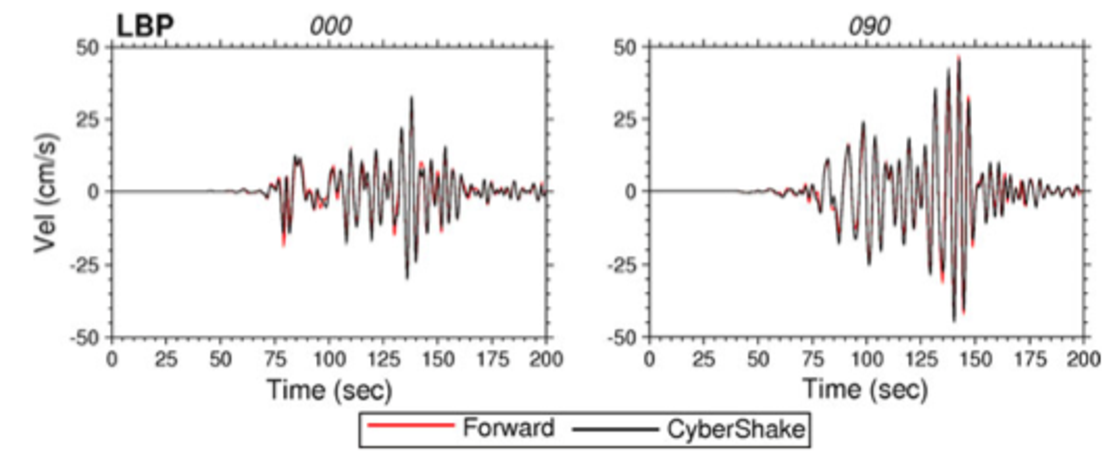
\includegraphics[height=4cm]{img/Inversion.pdf}
	\caption{Comparación de los resultados arrojados por la simulación de una ruptura de la falla de San Andrés que genera un sismo de $M_W=7\.8$. Rojo: Modelación directa, Negra: Reciprocidad sobre el Tensor de Deformaciones de Green \cite[figura 5, página 7]{gravesetal}}
	\vspace{-.5 cm}
\end{figure}
%
\justifying
Una forma de calcular el Tensor de Deformaciones de Green en los puntos en los cuales se discretizan las fallas, es calculando las derivadas numéricas respecto a las coordenadas espaciales del campo de desplazamientos generado por la carga unitaria aplicada en el sitio sobre el cual se quiere conocer la respuesta sísmica.\\
%
Trabajando con un Software de Elementos Finitos, es posible calcular directamente el Tensor de Desplazamientos sin necesidad de recurrir a la derivación numérica.
%
%
\end{frame}
%
%
%\section{Mapas de Amenaza Sísmica}
%\subsection{Curvas de Amenaza}
\begin{frame}[allowframebreaks]
\frametitle{Curvas de Amenaza}
%
Las curvas de amenaza presentadas, han sido calculadas empleando las GMPE de Boore y Atkinson (2008), Campbell y Bozorgnia (2009) y con la plataforma CyberShake.
%
\begin{figure}[h]
	\centering
	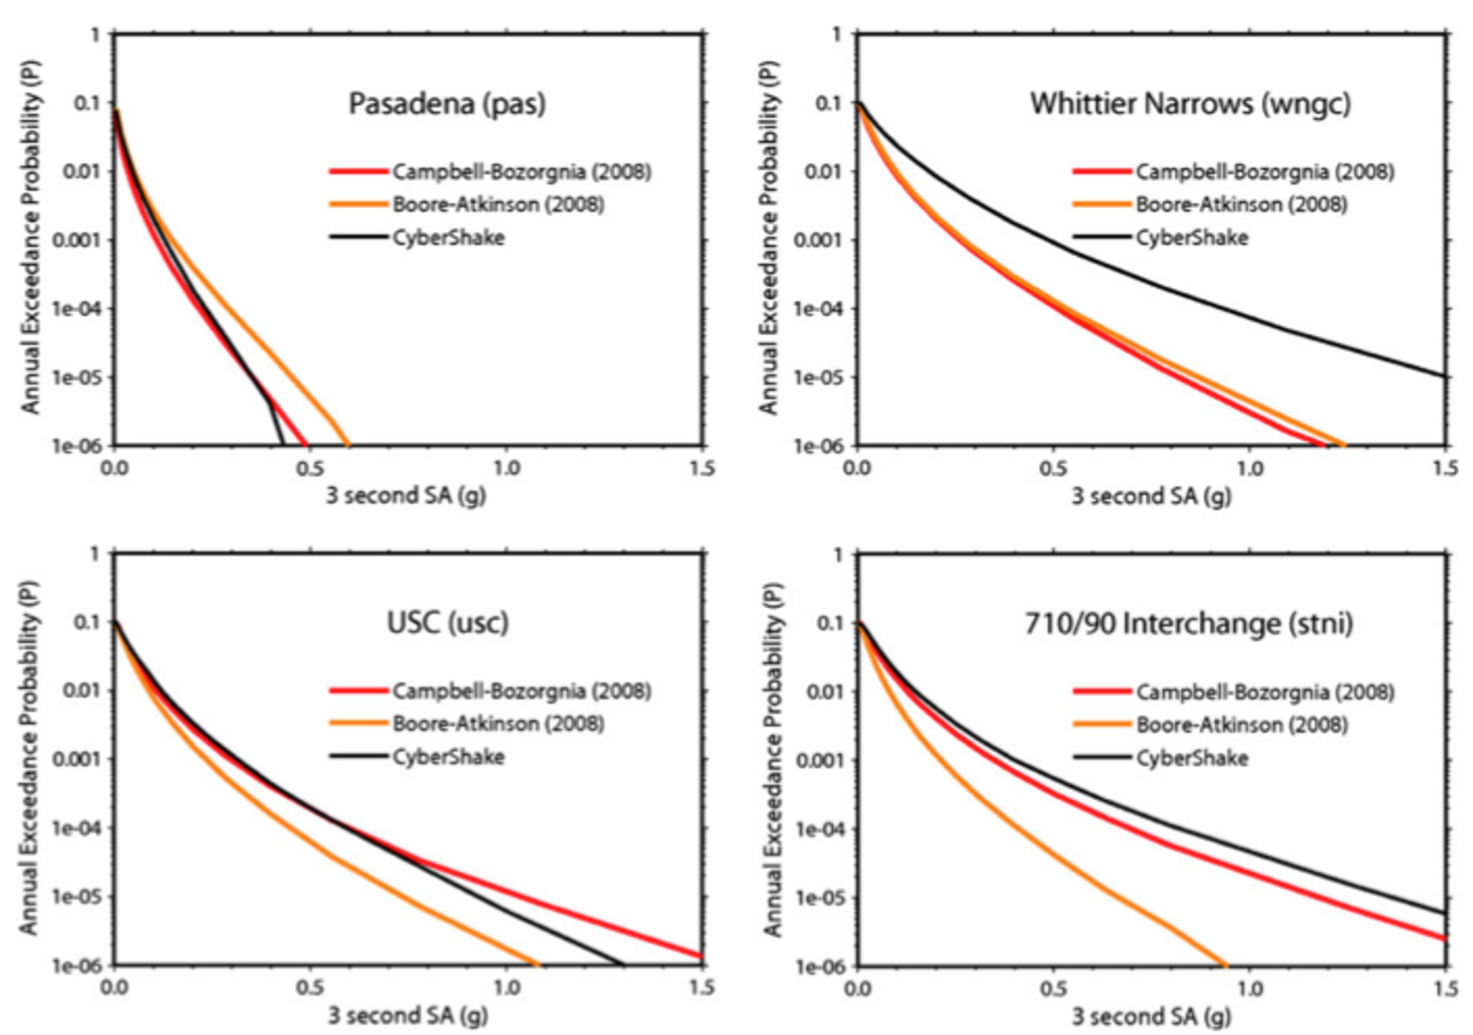
\includegraphics[height=5cm]{img/CurvasAmenaza.pdf}
	\caption{Curvas de Amenaza calculadas con dos leyes de atenuación y CyberShake \cite[figura 7, página 10]{gravesetal}}
	\vspace{-.5 cm}
\end{figure}
%
\justifying
%
Ambas GMPE utilizan el $V_{s30}$ (velocidad de viaje de las ondas sísmicas en los $30$m superiores) para tener en cuenta los efectos de sitio.\\
%
Las curvas de amenaza halladas para los movimientos del suelo encontrados con CyberShake, son calculadas con el software disponible en \url{http://www.opensha.org}, el cual combina la amplitud del movimiento del suelo con las probabilidades de ruptura especificadas en $UCERF2\.0$ y $UCERF3\.0$.
%
%
\end{frame}
%
%
%\subsection{Mapas de Amenaza}
\begin{frame}[allowframebreaks]
\frametitle{Mapas de Amenaza}
%
\justifying
%
Por último, para generar los mapas de amenaza sísmica con CyberShake, se lleva a cabo el siguiente procedimiento:
%
\begin{itemize}
%
	\item Cálculo del mapa de amenaza sísmica con las GMPE.
	%
	\item Cálculo de las curvas de amenaza con los movimientos del suelo hallados con CyberShake. Actualmente esta información se tiene en $250$ sitios.
	%
	\item Cálculo del residuo entre curvas de amenaza de las GMPE y CyberShake.
	%
	\item Los residuos del punto anterior se interpolan en toda la región de estudio.
	%
	\item Al mapa de amenaza calculado con las GMPE se les suma el residuo interpolado y se encuentra el Mapa de Amenaza calculado con CyberShake. 
%
\end{itemize}
%
\begin{figure}[h]
	\centering
	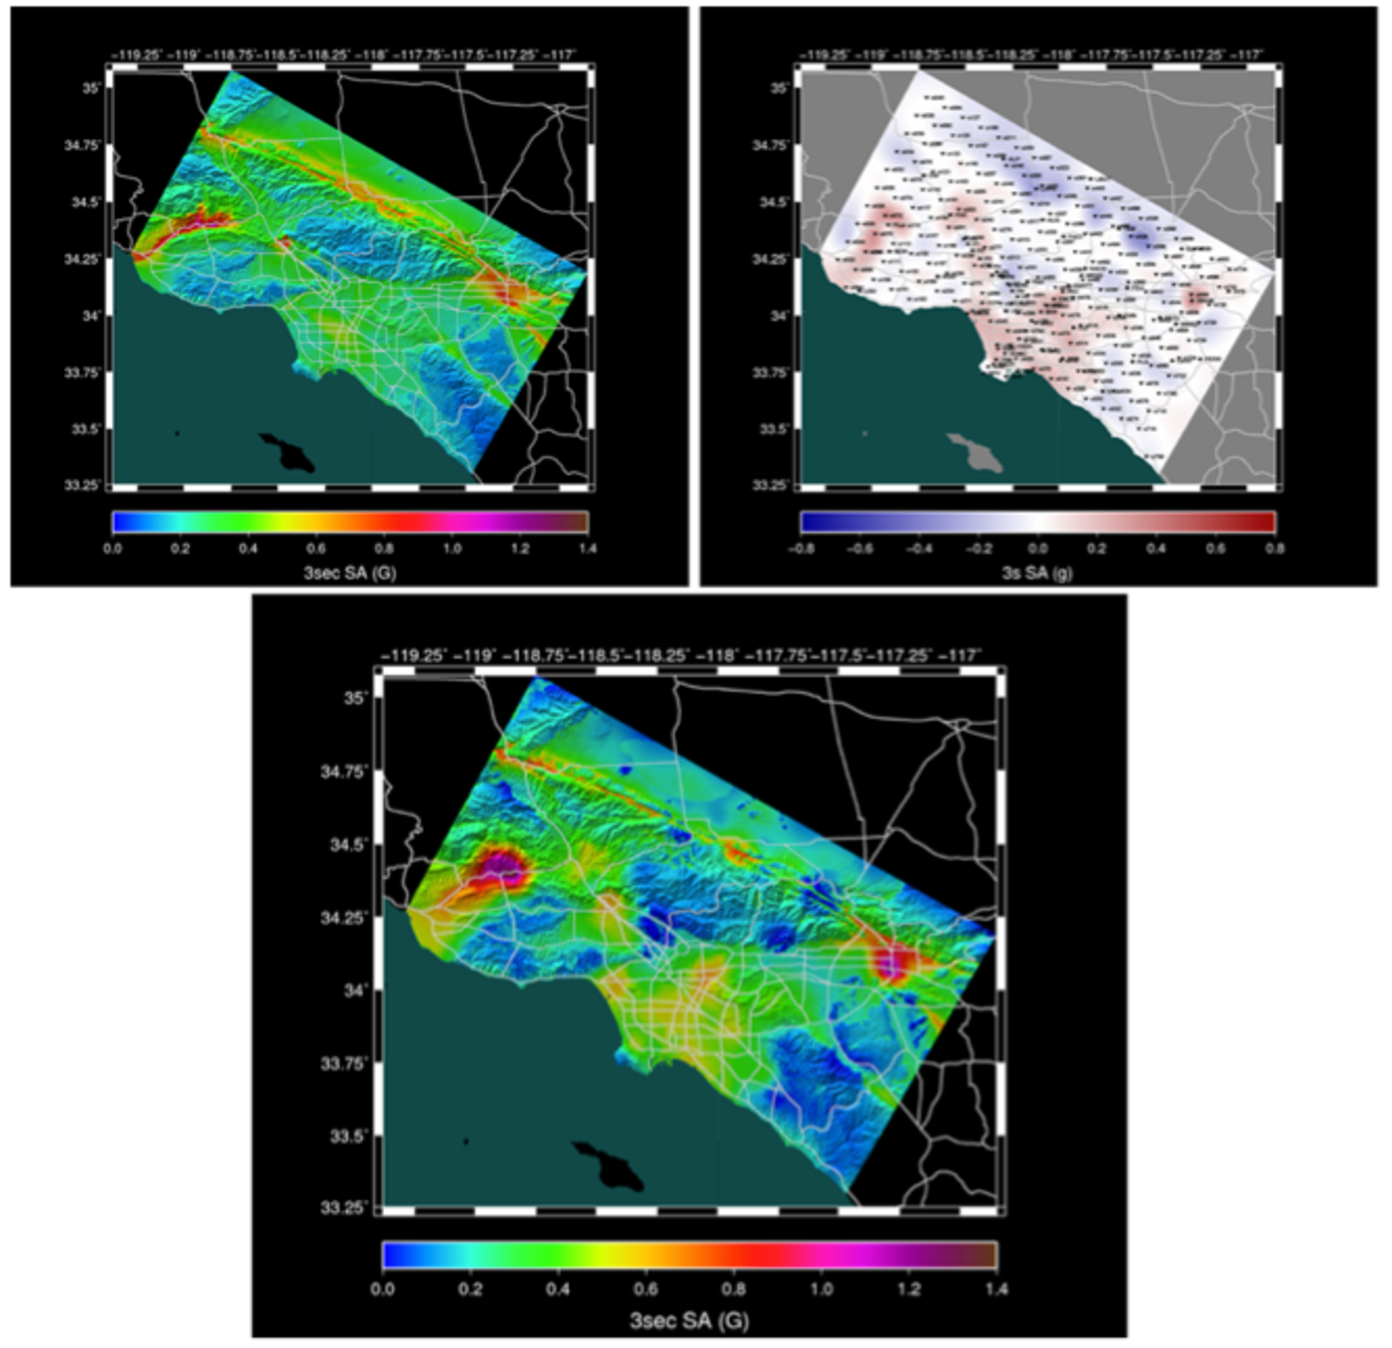
\includegraphics[height=5.5cm]{img/ProcesoMapaAmenaza.pdf}
	\caption{Procedimeinto calculo mapas de amenaza con CyberShake \cite[figura 9, página 12]{gravesetal}}
	\vspace{-.5 cm}
\end{figure}
%
\begin{figure}[h]
	\centering
	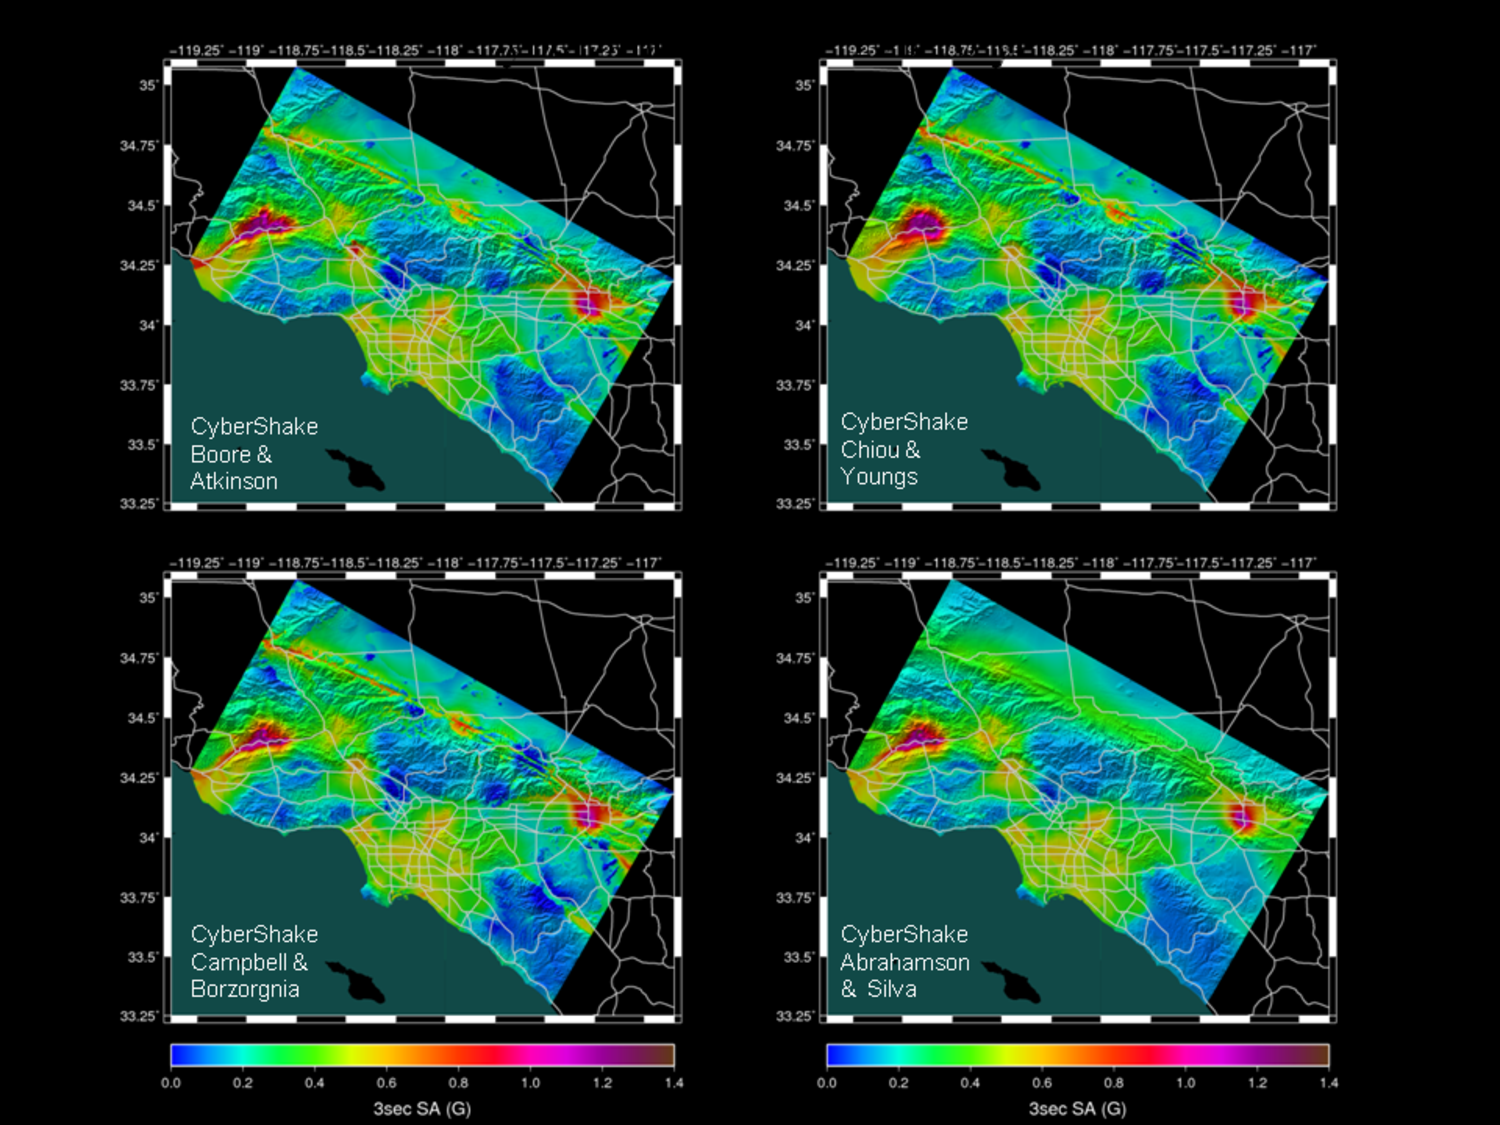
\includegraphics[height=5cm]{img/MapaAmenaza.pdf}
	\caption{Mapas de Amenaza con CyberShake construido con $4$ Leyes de Atenuación Diferentes \footnote{\tiny \url{http://scec.usc.edu/scecwiki/images/a/ad/UCERF2_WaveProp_2009.PNG}}}
	\vspace{-.5 cm}
\end{figure}
%
%
\end{frame}
%
%
%\section{Conclusiones}
\begin{frame}[allowframebreaks]
\frametitle{Conclusiones}
%
\justifying
%
Acá van las conclusiones
%
\end{frame}
%
%
\begin{frame}[allowframebreaks]{References}
\def\newblock{}
%\bibliographystyle{gji}
%\bibliography{refSCEC}
\bibliographystyle{plain}
\begin{thebibliography}{1}

\bibitem{book:aki} Keiiti Aki \& Paul G. Richards. {Q}uantitative {S}eismology. University Sciencie Books, 2nd Edition, Mill Valley, San Diego, 2002.

\bibitem{book:pujol} Jose Pujol. Elastic Wave Propagation and Generation in Seismology. Cambridge University Press, 1st Edition, Cambridge, United Kingdom, 2003.

\bibitem{baker} Baker, J. W., Luco, N., Abrahamson, N. A., Graves, R. W., Maechling, P. J., \& Olsen, K. B. (2014, July). Engineering Uses of Physics-based Ground Motion Simulations. In Proceedings of the Tenth US Conference on Earthquake Engineering.

\bibitem{gravesetal} Graves, R.; Jordan, T. H.; Callaghan, S.; Deelman, E.; Field, E.; Juve, G.; ... \& Vahi, K. (2011). CyberShake: A physics-based seismic hazard model for southern California. Pure and Applied Geophysics, 168(3-4), 367-381.

\bibitem{gravesgreen} Graves, R.; \& Wald, D. J. (2001). Resolution analysis of finite fault source inversion using one and three dimensional Green's functions: 1. Strong motions. Journal of Geophysical Research: Solid Earth (1978–2012), 106(B5), 8745-8766.

\bibitem{ucerf2} Field, E. H., Dawson, T. E., Felzer, K. R., Frankel, A. D., Gupta, V., Jordan, T. H., ... \& Wills, C. J. (2009). Uniform California earthquake rupture forecast, version 2 (UCERF 2). Bulletin of the Seismological Society of America, 99(4), 2053-2107.

\bibitem{ucerf3} Field, E.H., Biasi, G.P., Bird, P., Dawson, T.E., Felzer, K.R., Jackson, D.D., Johnson, K.M., Jordan, T.H., Madden, C., Michael, A.J., Milner, K.R., Page, M.T., Parsons, T., Powers, P.M., Shaw, B.E., Thatcher, W.R., Weldon, R.J., II, and Zeng, Y., 2013, Uniform California earthquake rupture forecast, version 3 (UCERF3)—The time-independent model: U.S. Geological Survey Open-File Report 2013–1165, 97 p., California Geological Survey Special Report 228, and Southern California Earthquake Center Publication 1792, \url{http://pubs.usgs.gov/of/2013/1165/}.

\bibitem{zhaogreen} Zhao, L., Chen, P., \& Jordan, T. H. (2006). Strain Green’s tensors, reciprocity, and their applications to seismic source and structure studies. Bulletin of the Seismological Society of America, 96(5), 1753-1763.

\end{thebibliography}

\end{frame}


\end{document}

